\documentclass[compress,10pt]{beamer}
% version imprimable pour assistance
%\documentclass[10pt, green, handout]{beamer}
\usepackage[T1]{fontenc}
\usepackage[utf8]{inputenc}
\usepackage[frenchb]{babel} % le document est en français
\usepackage{rotating,amsmath}
\usepackage{graphicx,cancel}       % pour ins\'erer des figures
        % pour d\'efinir plus de couleurs
\usetheme[outer/progressbar=foot]{metropolis}
\setbeamertemplate{section in toc}[sections numbered]
\setbeamertemplate{subsection in toc}[subsections numbered]

%\usetheme{metropolis}  %Applique le theme INRA (ce dernier doit être present dans le repertoire courant)
\usepackage{xcolor,colortbl}
\usepackage{array}
\usepackage{mdframed}
\usepackage{multirow}
\usepackage{lmodern}	
\usepackage{tikz}
\newcommand{\nodesize}{1.5em}
\newcommand{\edgeunit}{2*\nodesize}
\tikzstyle{hidden}=[draw, circle, fill=gray!50, minimum width=\nodesize, inner sep=0]
\tikzstyle{observed}=[draw, circle, minimum width=\nodesize, inner sep=0]
\tikzstyle{diagobserved}=[draw, circle, minimum width=\nodesize, inner sep=0,color=gray!50]
\tikzstyle{eliminated}=[draw, circle, minimum width=\nodesize, color=gray!50, inner sep=0]
\tikzstyle{empty}=[]
\tikzstyle{arrow}=[->, >=latex, line width=1pt]
\tikzstyle{edge}=[-, line width=1pt]
\tikzstyle{dashedarrow}=[->, >=latex, dashed, line width=1pt]
\tikzstyle{lightarrow}=[->, >=latex, line width=1pt, fill=gray!50, color=gray!50]



\usetikzlibrary{positioning,shapes,arrows}



\setbeamerfont{bibliography item}{size=\tiny}
\setbeamerfont{bibliography entry author}{size=\tiny}
\setbeamerfont{bibliography entry title}{size=\tiny}
\setbeamerfont{bibliography entry location}{size=\tiny}
\setbeamerfont{bibliography entry note}{size=\tiny}
            

\definecolor{dgreen2}{RGB}{102,193,191}
%RGB()
\definecolor{dgreen}{RGB}{255,165,0}
\definecolor{mygrey}{RGB}{230,230,230}


\setbeamertemplate{blocks}[rounded][shadow=true]
\setbeamercolor{block title}{use = structure  ,bg=mygrey, fg=dgreen}
%\setbeamercolor{normal text}{fg=black,bg=white}
%\setbeamercolor{alerted text}{fg=lgreen}
%\setbeamercolor{example text}{fg=lgreen}
%\setbeamercolor{structure}{fg=dgreen} %d'où ce bleu par défaut
\setbeamercolor{background canvas}{parent=normal text}


\usepackage{tikz}
\usetikzlibrary{calc,shapes,backgrounds,arrows,automata,shadows,positioning}
\setbeamertemplate{frametitlecontinuation}{\insertcontinuationcountroman}

%-------------------------------------------------------------------------------
% Quelques options pdf
%-------------------------------------------------------------------------------
\hypersetup{
pdfpagemode = FullScreen, % afficher le pdf en plein \'ecran
pdfauthor   = {},%
pdftitle    = {},%
pdfsubject  = {},%
pdfkeywords = {Science,Impact},%
pdfcreator  = {PDFLaTeX,emacs,AucTeX},%
pdfproducer = {INRAE}%
}


\newcommand\Wider[2][3em]{%
\makebox[\linewidth][c]{%
  \begin{minipage}{\dimexpr\textwidth+#1\relax}
  \raggedright#2
  \end{minipage}%
  }%
}

\AtBeginSection[]
{  \begin{frame}
  \frametitle{}
  \tableofcontents[currentsection, hideothersubsections]
  \end{frame} 
}
  \AtBeginSubsection[]
  {  \begin{frame}
    \frametitle{}
    \tableofcontents[currentsubsection, currentsection,hideothersubsections, subsectionstyle=show/shaded/hide]
    \end{frame} 
  }










%------------------------------------------
\title{Mathématiques pour l'écologie}
\subtitle{Simuler des écosystèmes désertiques}
\date{}
%\date{\emph{Journée des Jeunes Chercheur.e.s en Biométrie - Société Française de Biométrie}}, 
%Janvier 2023, Rennes (France)}}
\author{Sophie Donnet (INRAE)}
\titlegraphic{\hfill
\includegraphics[width= 0.3  \textwidth]{images/Logo-INRAE}}




\newtheorem{proposition}{Proposition}
\newtheorem{Remark}{Remark}


\newcommand{\cst}{\mbox{Cste}} 
\newcommand{\Zcal}{\mathcal{Z}}
\newcommand{\Esp}{\mathbb{E}}
\newcommand{\Espt}{\widetilde{\Esp}}
\newcommand{\It}{\widetilde{I}}
\newcommand{\Dcal}{\mathcal{D}}
\newcommand{\Qcal}{\mathcal{Q}}
\newcommand{\Mcal}{\mathcal{M}}
\newcommand{\Ecal}{\mathcal{E}}
\newcommand{\Ncal}{\mathcal{N}}
\newcommand{\Pcal}{\mathcal{P}}
\newcommand{\Var}{\mathbb{V}}
\newcommand{\Vart}{\widetilde{\Var}}
\newcommand{\diag}{\text{diag}}
\renewcommand{\vec}{\text{vec}}
\newcommand{\trans}{{\intercal}}



\newcommand{\ind}{\mathds{1}}
\newcommand{\btheta}{\theta}
\newcommand{\bY}{Y}
\newcommand{\bZ}{Z}
 
\newcommand{\papprox}{\pt_{\bY}}
\newcommand{\papproxs}{\pt_{\bY^{(s)}}}
\newcommand{\pexact}{p_{\bY}}
\renewcommand{\d}{\text{ d}}
\newcommand{\pbar}{\overline{p}}
\newcommand{\gammabar}{\overline{\gamma}}


\newcommand{\bthetahm}{\bZ_h^m,\btheta_h^m}

\newcommand{\bthetahmoins}{\bZ_{h-1},\btheta_{h-1}}
\newcommand{\bthetahmoinsm}{\bZ_{h-1}^m,\btheta_{h-1}^m}
\newcommand{\bthetah}{\bZ_h,\btheta_h}
%\newcommand{\bthetahm}{\bZ_{h-1},\btheta_{h-1}}

%\newcommand{\bthetah}{\btheta^{(h-1)}}
\newcommand{\bthetak}{\bZ_{k},\btheta_{k}}
\newcommand{\bthetakmoins}{\bZ_{k-1},\btheta_{k-1}}

\newcommand{\bthetaz}{\bZ_{0},\btheta_{0}}
\newcommand{\bthetazh}{\bZ_{0:h},\btheta_{0:h}}
\newcommand{\bthetazm}{\bZ_{0}^m,\btheta_{0}^m}
\newcommand{\bthetazhmoinsm}{\bZ_{0:h-1}^m,\btheta_{0:h-1}^m}
\newcommand{\bthetazhm}{\bZ_{0:h}^m,\btheta_{0:h}^m}

\newcommand{\bthetazhmoins}{\bZ_{0:h-1},\btheta_{0:h-1}}
 
\newcommand{\wb}{\overline{w}}
\newcommand{\wtilde}{\widetilde{w}}

\newcommand{\wh}{w_h}
\newcommand{\whm}{w_h^m}
\newcommand{\Whm}{W_h^m}
\newcommand{\Wh}{W_h}

\newcommand{\whmm}{w_{h-1}^m}
\newcommand{\Whmm}{W_{h-1}^m}
\newcommand{\SBMreg}{SBM-reg\xspace}
\newcommand{\SBS}{SBS\xspace}
\newcommand{\CBS}{CBS\xspace}
\newcommand{\CBSIS}{CBS$+$IS\xspace}



\newcommand{\alphat}{\widetilde{\alpha}}
\newcommand{\gammat}{\widetilde{\gamma}}
\newcommand{\betat}{\widetilde{\beta}}
\newcommand{\nut}{\widetilde{\nu}}
\newcommand{\thetat}{\widetilde{\theta}}
\newcommand{\ph}{p_h}
\newcommand{\qh}{q_h}
\newcommand{\rhoh}{\rho_h}
\newcommand{\qapprox}{\pt}
\newcommand{\vs}{\vspace{1em}}

\newcommand{\alphakl}{{\alpha_{k\ell}}}
\newcommand{\alphakkll}{\alpha_{k'\ell'}}
\newcommand{\betar}{\beta_r}
\newcommand{\et}{\widetilde{e}}
\newcommand{\nuk}{\nu_k}
\newcommand{\nul}{\nu_\ell}
\newcommand{\nuK}{\nu_K}
\newcommand{\numK}{\nu^{-K}}
\newcommand{\qt}{\widetilde{q}}
\newcommand{\pt}{\widetilde{q}}
\newcommand{\Vt}{\widetilde{V}}
\newcommand{\etaijkl}{\eta_{ij}^{k\ell}}
\newcommand{\tauik}{\tau_{ik}}
\newcommand{\tauil}{\tau_{i\ell}}
\newcommand{\tauiK}{\tau_{iK}}
\newcommand{\taujl}{\tau_{j\ell}}
\newcommand{\taupk}{\tau_{+k}}
\newcommand{\taupK}{\tau_{+K}}
\newcommand{\taumK}{\tau^{-K}}
\newcommand{\taut}{\widetilde{\tau}}
\newcommand{\tautik}{\taut_{ik}}
\newcommand{\tautil}{\taut_{i\ell}}
\newcommand{\tautiK}{\taut_{iK}}
\newcommand{\tautjl}{\taut_{j\ell}}
\newcommand{\tautpk}{\taut_{+k}}
\newcommand{\tautpK}{\taut_{+K}}
\newcommand{\tautmK}{\taut^{-K}}
\newcommand{\xij}{x_{ij}}
\newcommand{\Yij}{Y_{ij}}
\newcommand{\Zik}{Z_{ik}}
\newcommand{\Zuk}{Z_{uk}}
\newcommand{\ZiK}{Z_{iK}}
\newcommand{\Zjl}{Z_{j\ell}}
\newcommand{\Zul}{Z_{u\ell}}
\newcommand{\Zvl}{Z_{v\ell}}
\newcommand{\Zvm}{Z_{vm}}
% \newcommand{\Nk}{Z_{+k}}
% \newcommand{\Nl}{Z_{+\ell}}
% \newcommand{\NK}{Z_{+K}}
\newcommand{\Nk}{N_k}
\newcommand{\Nl}{N_\ell}
\newcommand{\NK}{N_K}
\newcommand{\Ntk}{\widetilde{N}_k}
\newcommand{\Ntl}{\widetilde{N}_\ell}
\newcommand{\NtK}{\widetilde{N}_K}
\newcommand{\Stk}{\widetilde{S}_k}
\newcommand{\Stl}{\widetilde{S}_\ell}
\newcommand{\StK}{\widetilde{S}_K}
\newcommand{\Ctkl}{\widetilde{C}_{k\ell}}
\newcommand{\CtkK}{\widetilde{C}_{kK}}
\newcommand{\CtlK}{\widetilde{C}_{\ell K}}
\newcommand{\Dt}{\widetilde{D}}
\newcommand{\Et}{\widetilde{E}}

\newcommand{\pr}[1]{\mathbb{P}(#1)}
\newcommand{\emphase}[1]{\textcolor{dgreen}{#1}}

\newcommand{\ra}{\bigskip \textcolor{dgreen}{$\rightarrow$}\;}

\newcommand{\ts}{{\theta^{*}}}
\newcommand{\kl}{{(k\ell)}}


\newcommand{\gv}{\;|\;}
\newcommand{\PSBMreg}{Poisson SBM-reg\xspace}
\newcommand*\circled[1]{\tikz[baseline=(char.base)]{
            \node[shape=circle,draw,inner sep=1pt] (char) {#1};}}
            
\definecolor{darkgreen}{rgb}{0,0.4,0}
\newcommand{\red}[1]{\textcolor{red}{#1}}
\newcommand{\blue}[1]{\textcolor{blue}{#1}}
\newcommand{\gray}[1]{\textcolor{gray}{#1}}


\DeclareMathOperator*{\argmax}{argmax}
\DeclareMathOperator*{\argmin}{argmin}

\usepackage{amsmath}


%====================================================================
\begin{document}
\maketitle
%====================================================================
% \frame{ \frametitle{Présentation}
% 
% \begin{itemize}
%  \item Chercheuse en apprentissage statistique pour les sciences du vivant
%  \item Spécialisée en statistiques pour l'écologie
%  \item Unité MIA-Paris-Saclay, Campus Agronomique, INRAE
%  
%  \begin{center}
% 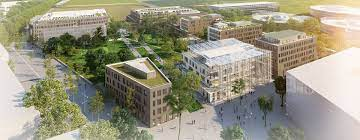
\includegraphics[width = 0.6 \textwidth]{images/Campus}  
%  \end{center}
%  
%  \item \textbf{Parcours}
%  \begin{itemize}
% \item  Classe préparatoire (MPSI-MP)
% \item L3,M1,M2 de mathématiques 
% \item Doctorat en mathématiques appliquées aux neurosciences
% \end{itemize}
% \end{itemize}
% }

% %====================================================================
% \frame{ \frametitle{Apprentissage statistique et écologie}
% %====================================================================
% 
% \begin{itemize}
%  \item \textbf{Apprentissage statistique} 
% \begin{itemize}
%  \item Art d'extraire de l'information d'un ensemble de données pour répondre à une question donnée
%  \item D'un calcul de moyenne à l'intelligence artificielle
% \end{itemize}
% \item \textbf{Ecologie}
% 
% \begin{itemize}
% \item Étude des milieux où vivent les êtres vivants, ainsi que des rapports de ces êtres avec le milieu et entre eux
% 
%  \begin{center}
% 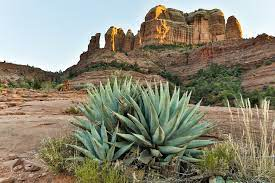
\includegraphics[width = 0.5 \textwidth]{images/ecosysteme}  
%  \end{center}
%  
%  
% \end{itemize}
% \end{itemize}
% 
% }
%====================================================================
\frame{\frametitle{Inspiré d'un travail multidisciplinaire}



\centering
\begin{tabular}{cccc}
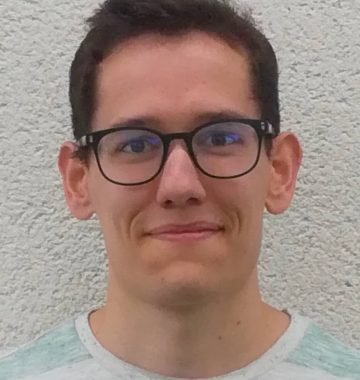
\includegraphics[width = 0.2 \textwidth]{images/Benoit}&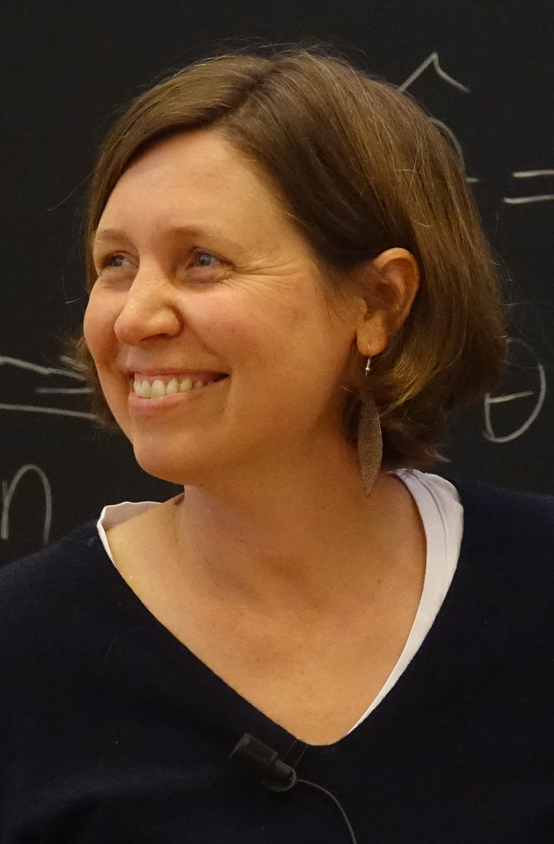
\includegraphics[width = 0.2 \textwidth]{images/sophie_donnet}&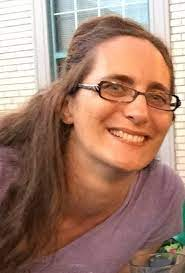
\includegraphics[width = 0.2 \textwidth]{images/Isabelle}&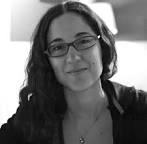
\includegraphics[width = 0.2 \textwidth]{images/Sonia}\\
\hline
B. Pichon & S. Donnet & I. Gounand & S. Kéfi\\
\hline 
 ISEM & MIA Paris Saclay & IEES & ISEM\\
 \hline
\end{tabular}
}

%===================================================================
\section{Introduction }
%====================================================================
\frame{\frametitle{Zones arides}
%====================================================================

\begin{itemize}
 \item Zones arides : environnements aux ressources limitées
 \item Végétation spatialement organisée

\end{itemize}
 \begin{center}
\begin{tabular}{cc}
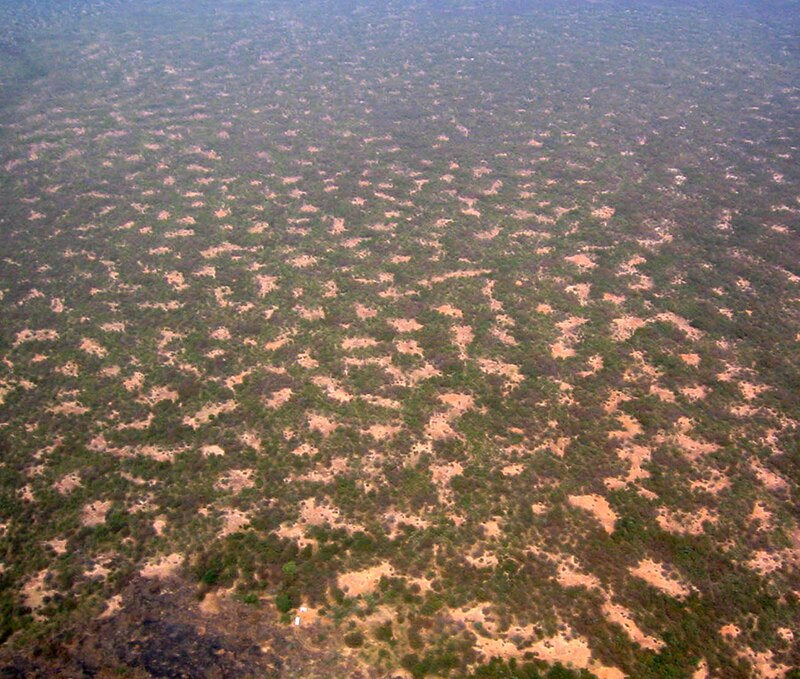
\includegraphics[width = 0.3 \textwidth]{images/Gapped_Bush_Niger_Nicolas_Barbier}&
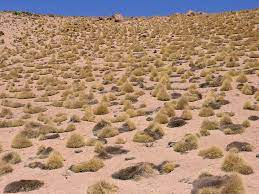
\includegraphics[width = 0.3 \textwidth]{images/pajabrava}\\
{\small Nigerian bush} &  {\small Departamento de Potosi, Bolivia}
\end{tabular}
\end{center}

Organisation est dûe à la biologie et notamment aux interactions entre plantes 
}
%====================================================================
\frame{\frametitle{Plantes tolérantes au stress}
%====================================================================
\begin{center}
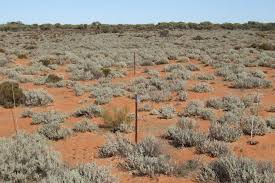
\includegraphics[width = 0.5 \textwidth]{images/stressTolerantPlant.jpeg}
\end{center}

 \begin{itemize}
 \item Facilitent leur environnement local en augmentant l'infiltration d'eau, en fournissant de l'ombre et en augmentant la disponibilité des nutriments locaux. \cite{choler_facilitation_2001,liancourt_stress_2005,flores_are_2003,he_testing_2012,qi_competitive_2018}
 \item Le mécanisme conduit à l’agrégation des plantes en patches séparés par des zones de sol nu (mosaïque à deux phases)
 \end{itemize} 
 }

 
%====================================================================
\frame{\frametitle{Objectifs du travail}
%====================================================================

Zones arides : des écosystèmes fragiles qui peuvent se dégrader brutalement


\textbf{Idée} : la répartition spatiale des plantes pourrait être un  indicateurs de l’approche des points de basculement vers la dégradation des écosystèmes


 \begin{center}
\begin{tabular}{cc}
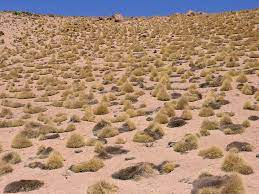
\includegraphics[width = 0.3 \textwidth]{images/pajabrava} & 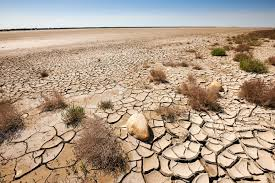
\includegraphics[width = 0.5 \textwidth]{images/desert_degraded}\end{tabular}
\end{center}


\textbf{But}: Utiliser ces motifs spatiaux pour estimer une distance à l'effondrement à partir  d'images satellites des zones arides
}

\section{Les données Biocom}

%====================================================================
\frame[allowframebreaks]{\frametitle{Les données Biocom.}
%====================================================================

\begin{itemize}
 \item 293 images réparties sur  115 sites autour du globe (13 countries)
 
 \begin{center}
  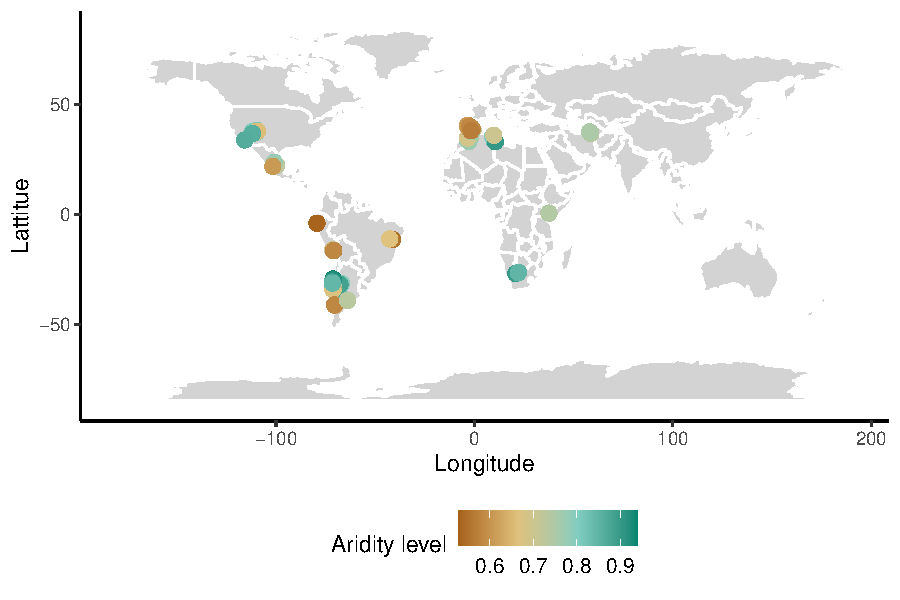
\includegraphics[width=0.6 \textwidth]{images/Map_empirical_sites.pdf} 
  \end{center}
  
 \item Paysages $50$m $\times$ $50$m 
 \item Résolution suffisante pour identifier les patches de végétation  (résolution spatiale $\leq$ 0.3 mètres par pixel).
\item Binarisation des images 
\end{itemize}
\begin{center}
 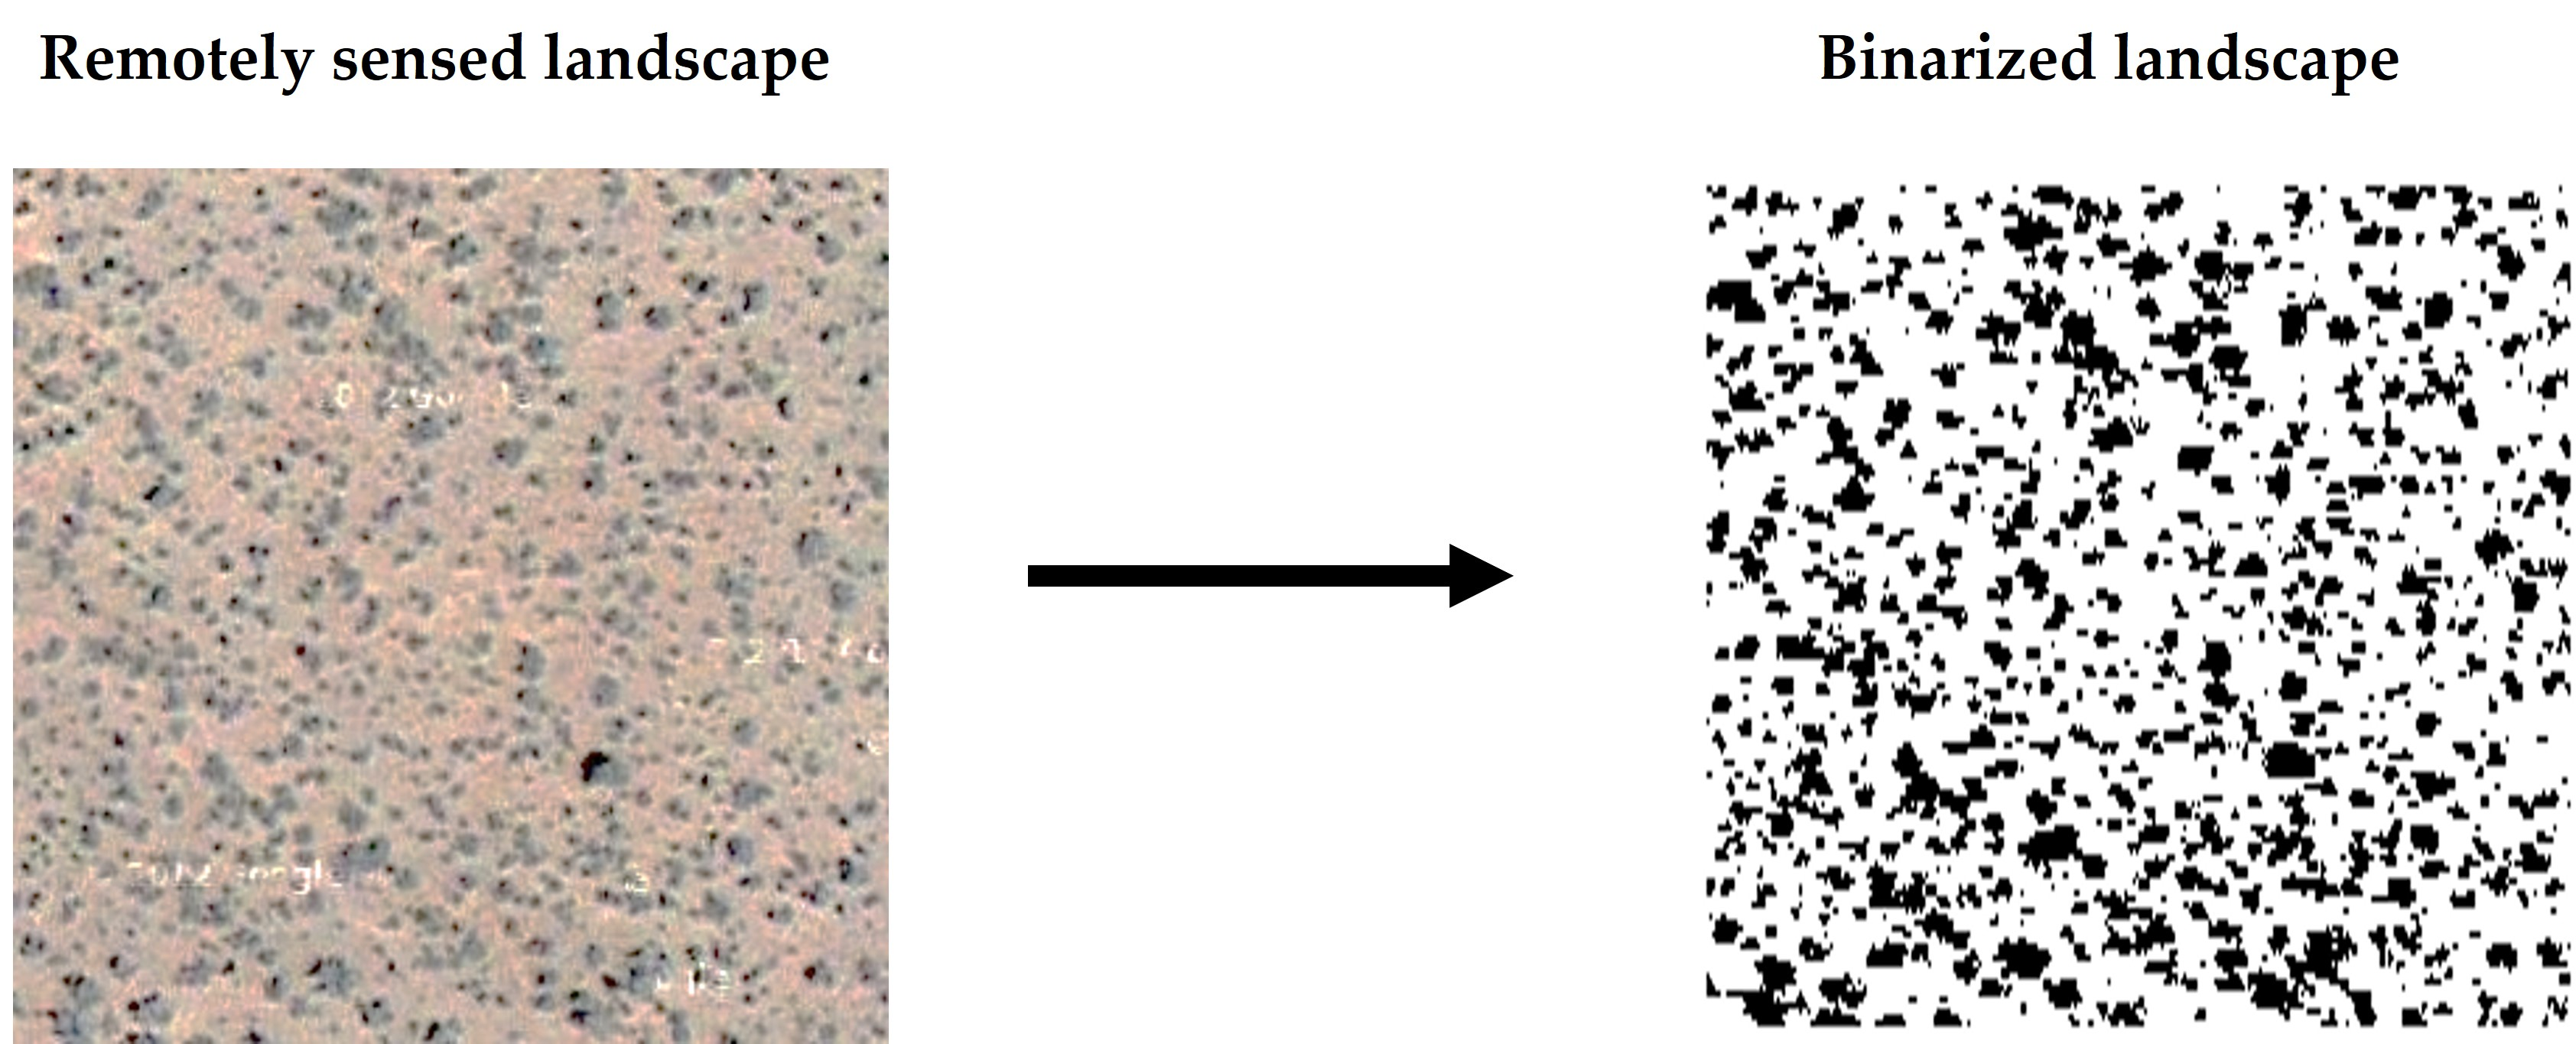
\includegraphics[width  = 0.8 \textwidth]{images/Binarization}
\end{center}
}


%====================================================================
\frame{\frametitle{Nos objectifs}
%====================================================================


\begin{block}{D'ici la fin de la semaine}
Ecrire un code Python qui permet de générer  des paysages désertiques
\end{block}


\begin{enumerate}
\item S'entraîner à Python, à l'aléatoire et à la modélisation sur un modèle de marche aléatoire (Lundi après midi -  mardi matin) 
 \item Coder un modèle biologique de paysages désertiques (voir plus tard)  (Mardi -  jeudi)  
 \item Comprendre comment il se comporte quand je change les paramètres  (Mardi -  jeudi)  
 \item $^\star$  Savoir si notre modèle s'adapte bien aux images qu'on a? 
 \end{enumerate}

}


\section{Un modèle minimal des dynamiques de végétation}

%====================================================================
\frame{\frametitle{Pourquoi un modèle}
%====================================================================

\begin{itemize}
 \item \textbf{Hypothèse}: chaque image est la réalisation d'un processus aléatoire qui obéit à des principes d'écologie
 \item Simplification de la réalité
 \item Suffisamment complexe pour représenter la réalité
\end{itemize}


}

%====================================================================
\frame{\frametitle{Notre modèle minimal}
%====================================================================
Variation autour de \cite{eby_alternative_2017,sankaran_clustering_2019}

\begin{itemize}
 \item Vise à imiter les écosystèmes stressés tels que les zones arides ou les marais salants :
 \item Automate cellulaire stochastique qui décrit l'évolution temporelle d'un paysage
 \item Image: $C \times C$ ($C = 100$) cellules qui peuvent se trouver dans deux états possibles $I_i(t)$.
\begin{itemize}
 \item soit colonisé par la végétation ($V$) 
 \item soit vide ($E$).
\end{itemize}
\item 1 cellule : une plante individuelle (typiquement dans les zones arides entre $0.25m^2$ et $1m^2$).
 \end{itemize}
}

%====================================================================
\frame{\frametitle{Un modèle à deux paramètres}
%====================================================================
A chaque pas de temps $t$, l'état des cellules $I_i(t)$ dans le paysage change en fonction de deux paramètres de probabilité : 

\begin{itemize}
 \item $p$ la reproduction locale de la végétation,
 \item $q$ un paramètre d'agrégation spatiale qui quantifie  l'auto-organisation spatiale.
\end{itemize}
}

%====================================================================
\frame{\frametitle{ $\forall i \mid  I_i(t) = V$} 
%====================================================================

Perform the following simulations 

\centering
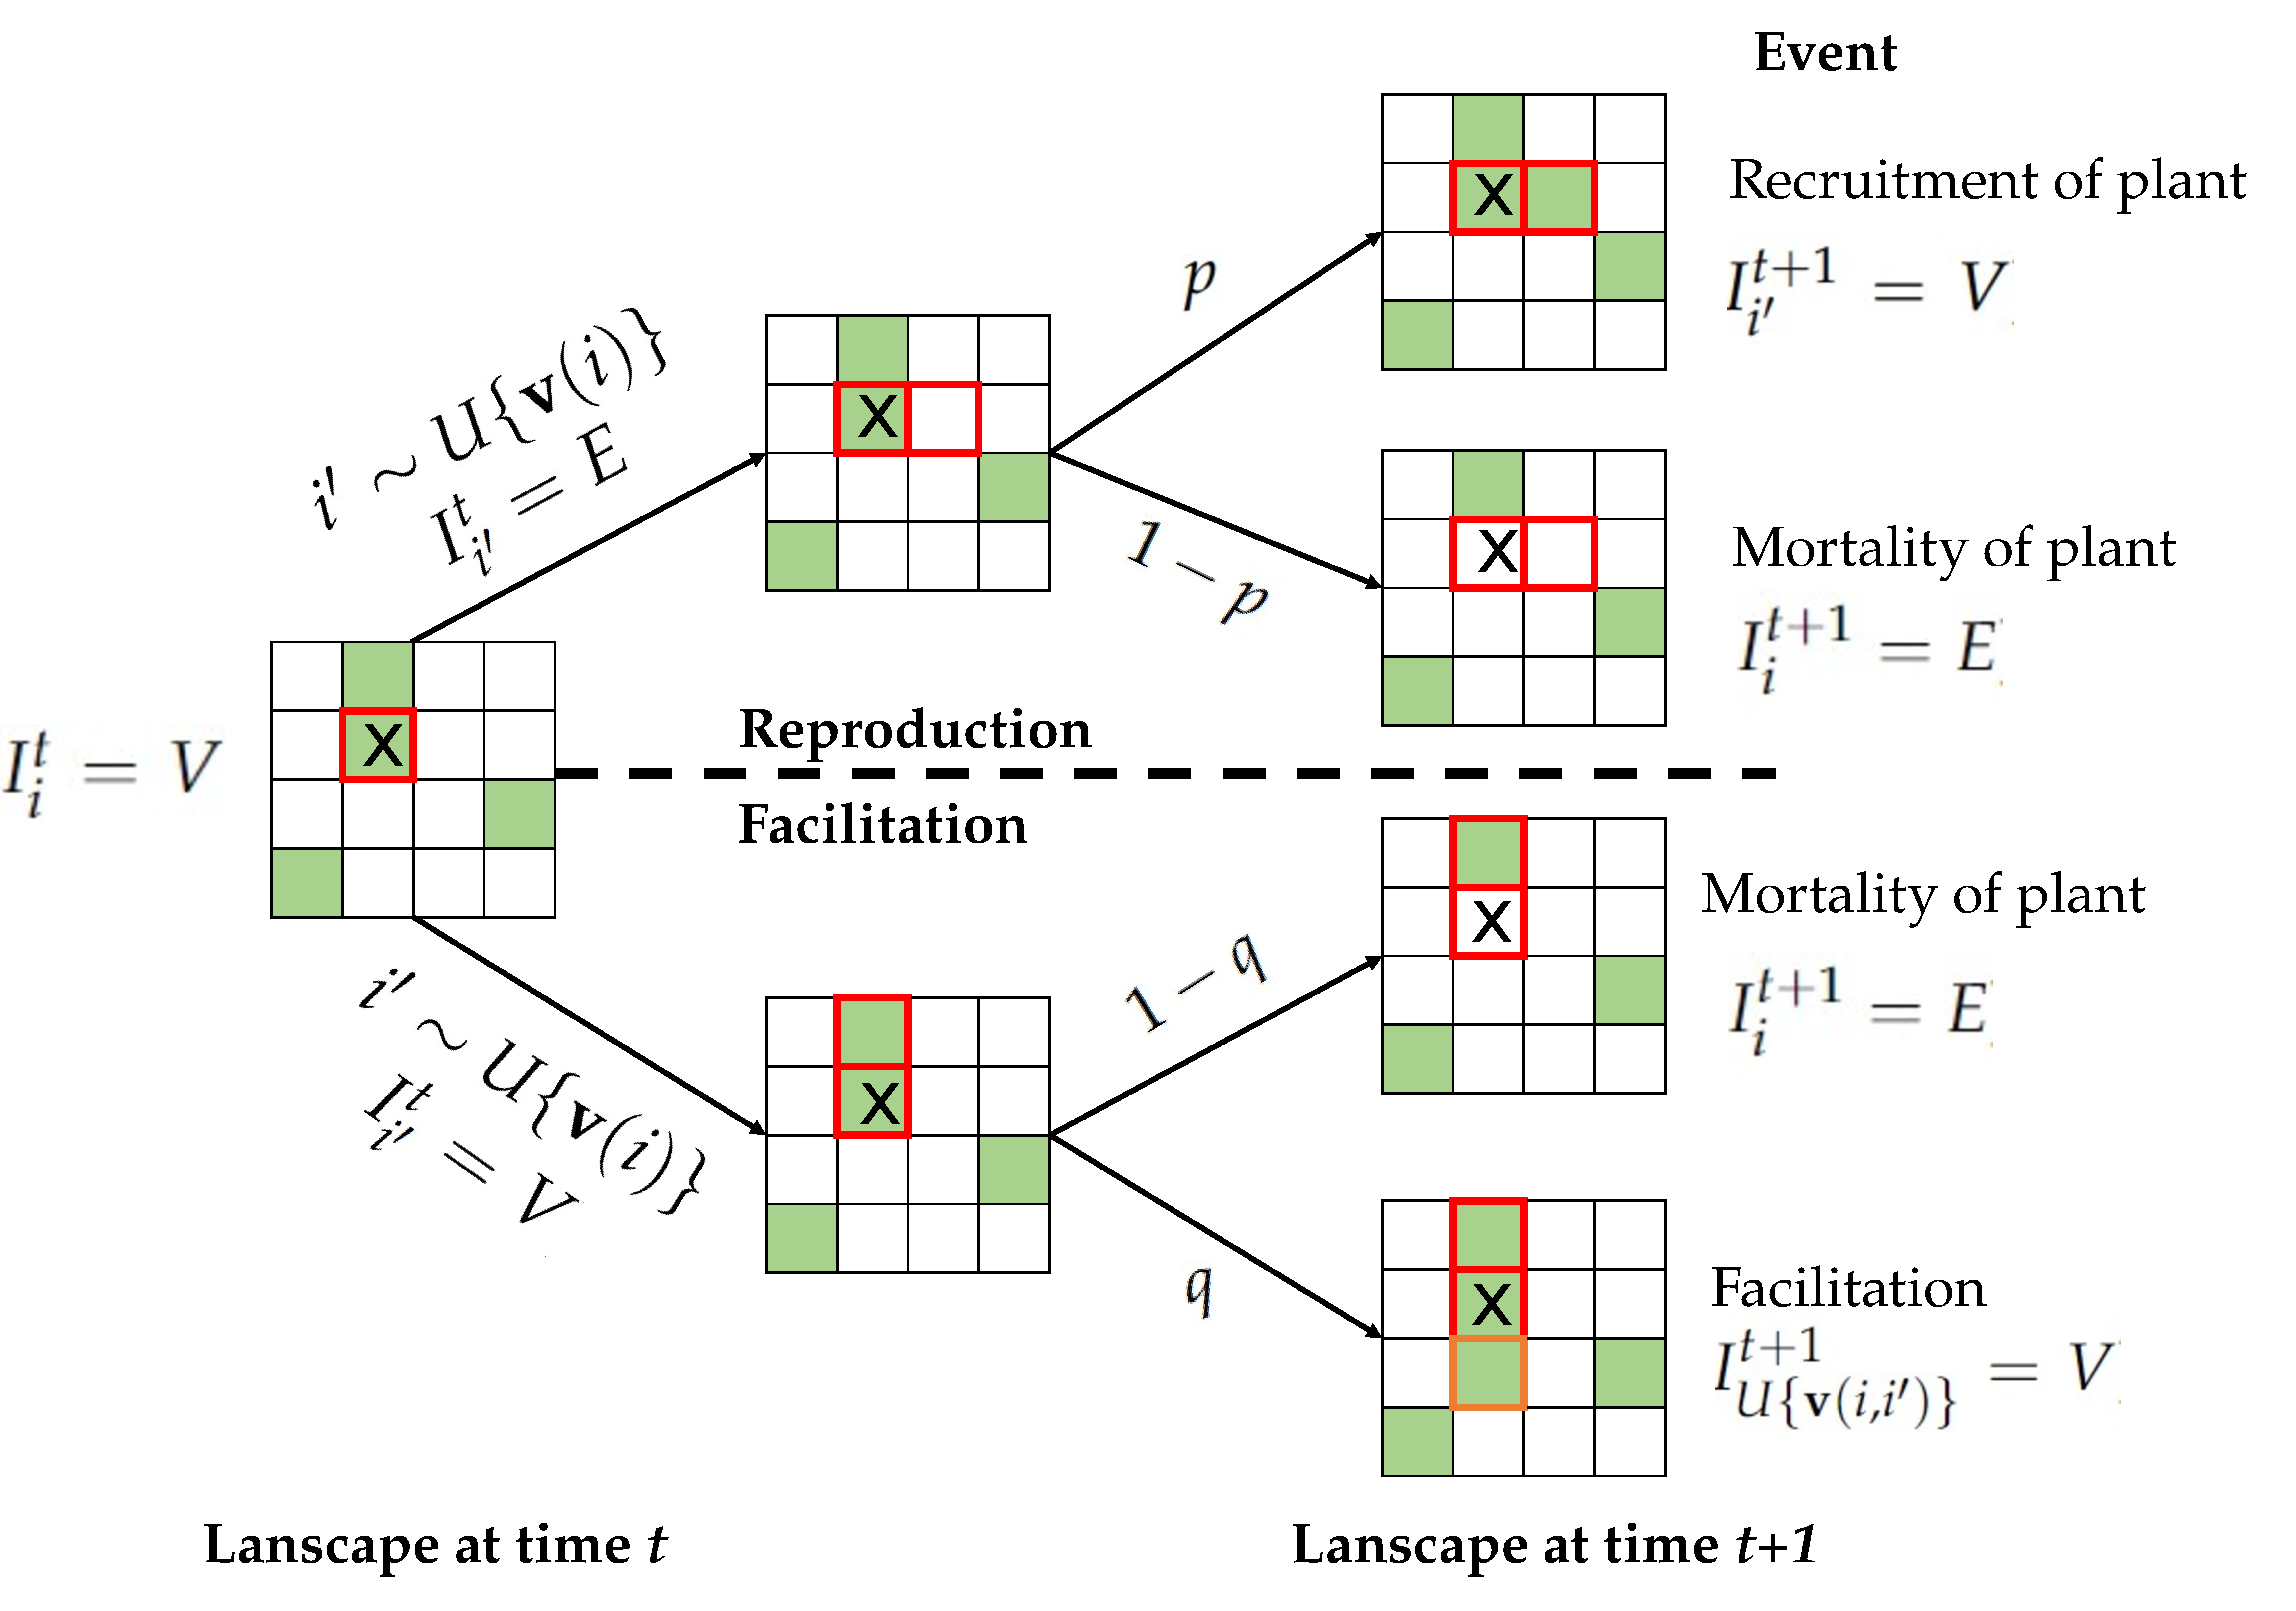
\includegraphics[width=0.8\textwidth]{images/model_description.pdf} 

jusqu'à stationarité
}

%====================================================================
\frame{\frametitle{Exemples of simulations} 
%====================================================================
\begin{tabular}{cc}
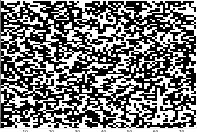
\includegraphics[width = 0.4 \textwidth, height = 0.4 \textwidth]{images/sim_model_1} 
&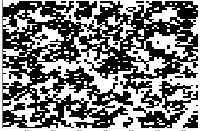
\includegraphics[width = 0.4 \textwidth, height = 0.4 \textwidth]{images/sim_model_2}\\
 $ \uparrow p$,  $\downarrow q$ & $\uparrow q$, $\downarrow p$ 
\end{tabular}

} 







% %====================================================================
% \frame{\frametitle{Additional descriptors}
% %====================================================================
% BIOCOM dataset: \cite{maestre_plant_2012,berdugo_plant_2017} Biotic and abiotic additional informations
%   \begin{itemize}
%   \item Soil sand content, 
%   \item Multifunctionality index (i.e., a $Z$-score of 16 soil variables associated with carbon, nitrogen and phosphorous cycling and storage etc)
%  \item Soil amelioration index, measured as the difference in organic carbon content between vegetated and bare soil areas
%  \item Level of facilitation (i.e., the proportion of plant species that are significantly more in the neighborhood of a facilitating species).
%  \end{itemize}
% }



%====================================================================
\frame{\frametitle{Echelle d'observation}
%====================================================================

\centering
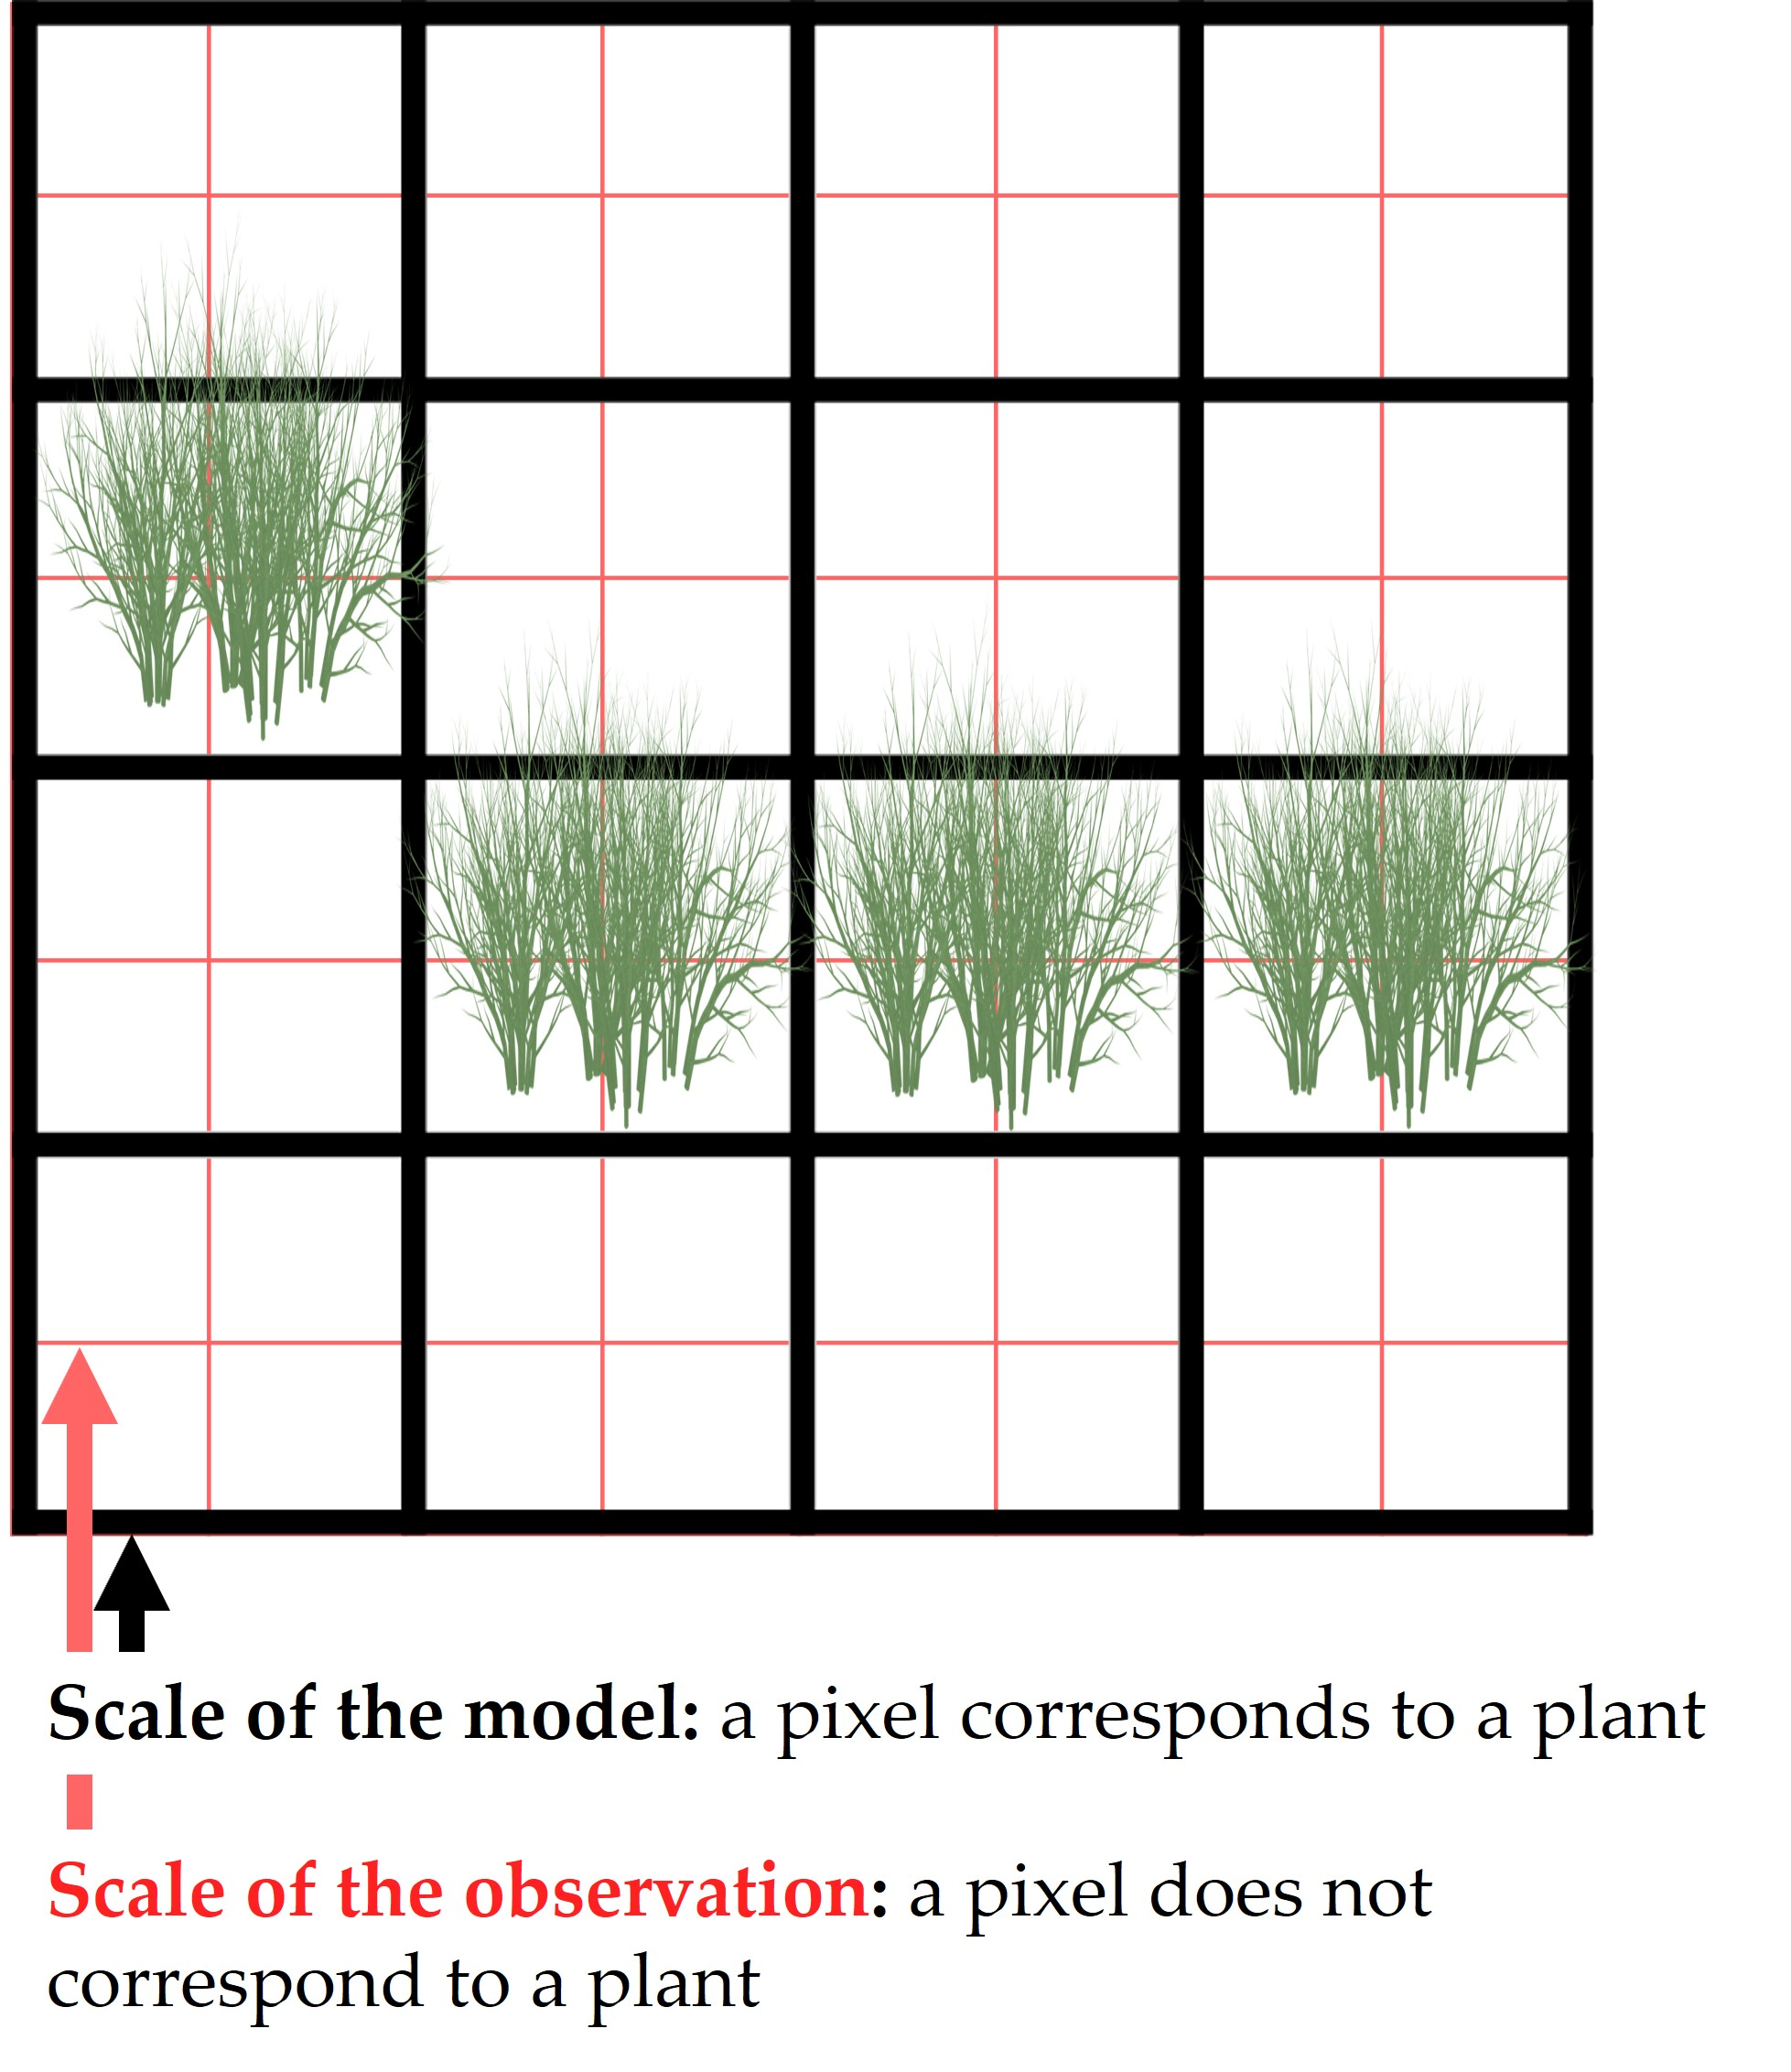
\includegraphics[width=0.5\textwidth]{images/scale_obs} \\

$\eta^2 $ : nombre de pixels inclus dans une cellule biologique. 

}

%====================================================================
\frame{\frametitle{Formalisation}
%====================================================================
Pour chaque photo $\ell$: 
\begin{eqnarray*}
 Y_{\ell,\bullet}(t) &=& F_\mathcal{O}(I_{\ell,\bullet}(t), \eta_\ell) \\
 I_{\ell,\bullet}(t) &\sim& \mathcal{M}_V(p_\ell,q_\ell) \\
 \theta_\ell &=& (p_\ell,q_\ell,\eta_\ell)
\end{eqnarray*}

\begin{itemize}
\item Model $\Mcal(\theta)$
\item ``Easy'' to simulate
\end{itemize}
}


%====================================================================
\frame{\frametitle{Estimation des paramètres}
%====================================================================
\centering
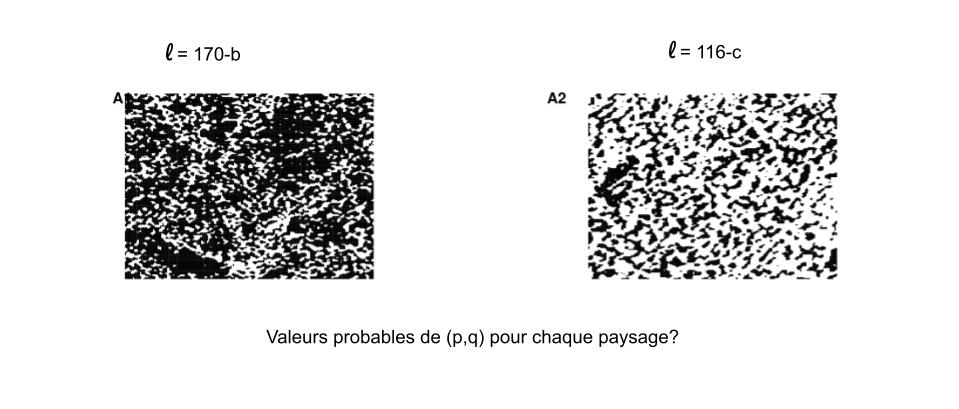
\includegraphics[width =  \textwidth]{images/Inference}

}


%====================================================================
\frame{\frametitle{ABC inference}
%====================================================================
\textbf{Approximate Bayesian Inference} 

Soit  $Y^{obs}$ l'image qui nous intéresse. 

\begin{block}{For all $m=1, \dots, M$ }
\begin{itemize}
\item Generation de paramètres ``au hasard''  $$\theta^{(m)} = (p^{(m)}, q^{(m)}, \eta^{(m)}) \sim \mbox{prior }$$ 
\item  Simulation de données fictives pour ces paramètres 
$$Y^{(m)} \mid \theta^{(m)} \sim \mathcal{M}(\theta^{(m)})$$


\begin{itemize}
\item Si l'image simulée ressemble à la ``vraie'' image, on garde le paramètre $\theta^{(m)}$, 
\item Sinon on le rejette
\end{itemize}

\end{itemize}
\end{block}



\begin{center}
L'échantillon obtenu ainsi est appelé \textbf{``échantillon sous la loi a posteriori''}
 
\end{center}


} 



%====================================================================
\frame{\frametitle{Comment quantifier la ressemblance?}
%====================================================================

\textbf{Définition d'une discrépance}


Repose sur  $11$ statistiques spatiales qui résument la complexité de la structuration spatiale.  


\begin{itemize}


   \item \textbf{Le couvert végétal}  (3 statistiques)
%   \begin{itemize}
%    \item vegetation cover ($S_1$) (fraction of vegetated sites),
%    \item $S_2$ the average number of plants in the neighborhood of each vegetation site (four nearest neighbors  \textit{i.e.} von Neumann neighborhood), 
%    \item as well as $S_3$, the log-transformed vegetation clustering (average number of neighbors divided by the vegetation cover).
%   \end{itemize}
%  
\item \textbf{L'aggrégation}  (4 statistics):  R-package \textsf{spatialwarnings} \cite{genin_monitoring_2018}.
\item \textbf{La distribution de la taille des patchs}  (4 statistiques)
\end{itemize}


 
% \textbf{Remarks}: Correlated but no selection was made
 
}

%====================================================================
\frame{\frametitle{Validation de la méthode d'inférence}
%====================================================================

Ici $M = 367500$

\begin{itemize}
 \item  On fabrique des fausses données $Y^{obs}$ sous notre modèle ou sous un autre
 \item Pour ces données on connait ses paramètres $p^\star,q^\star$
 \item On les oublie et on applique ABC pour essayer de les retrouver
 \item On valide la méthode d'inférence si on est capable de retrouver les paramètres
\end{itemize}



}

\section{Résultats  de l'inférence}

%====================================================================
\frame{\frametitle{Deux exemples de l'inférence a posteriori}
%====================================================================
\centering
    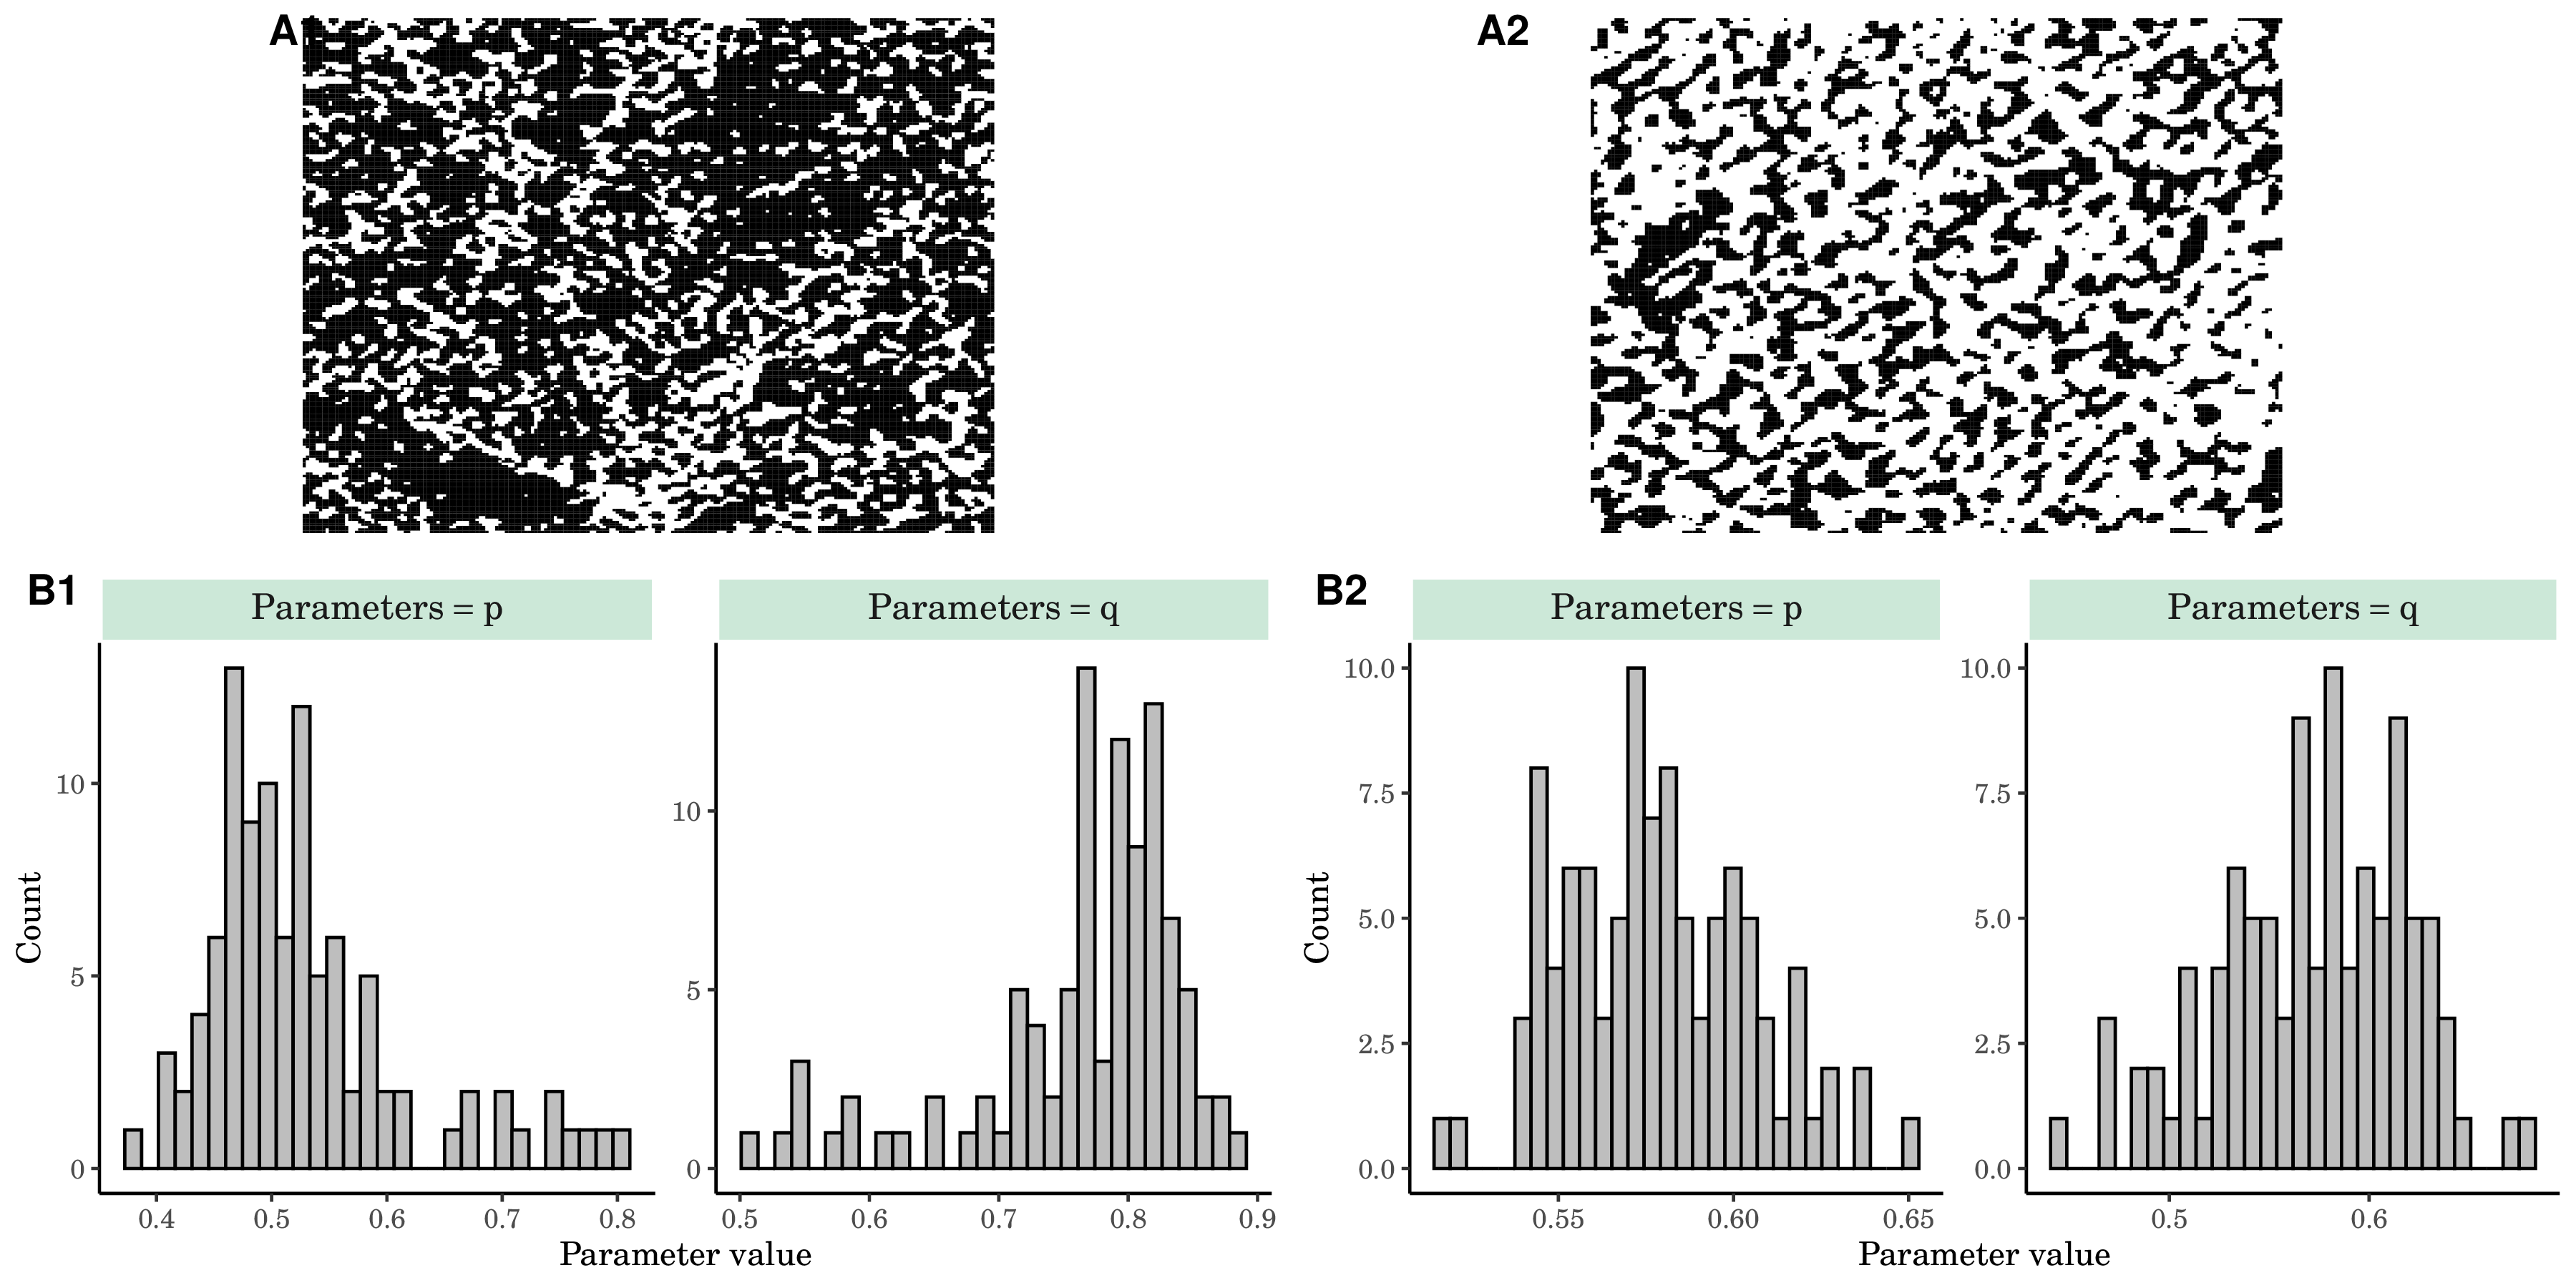
\includegraphics[width=\textwidth]{images/Example_sites_distrib} 

  {\small Exemples de distributions a posteriori des deux paramètres ($p$,$q$) pour deux sites à structure spatiale contrastée (170-b et 116-c de BIOCOM  \cite{miguel_berdugo_data_2017})}.
}



%====================================================================
\frame{\frametitle{Simulation sour la loi prédictive a posteriori}
%====================================================================

\centering
    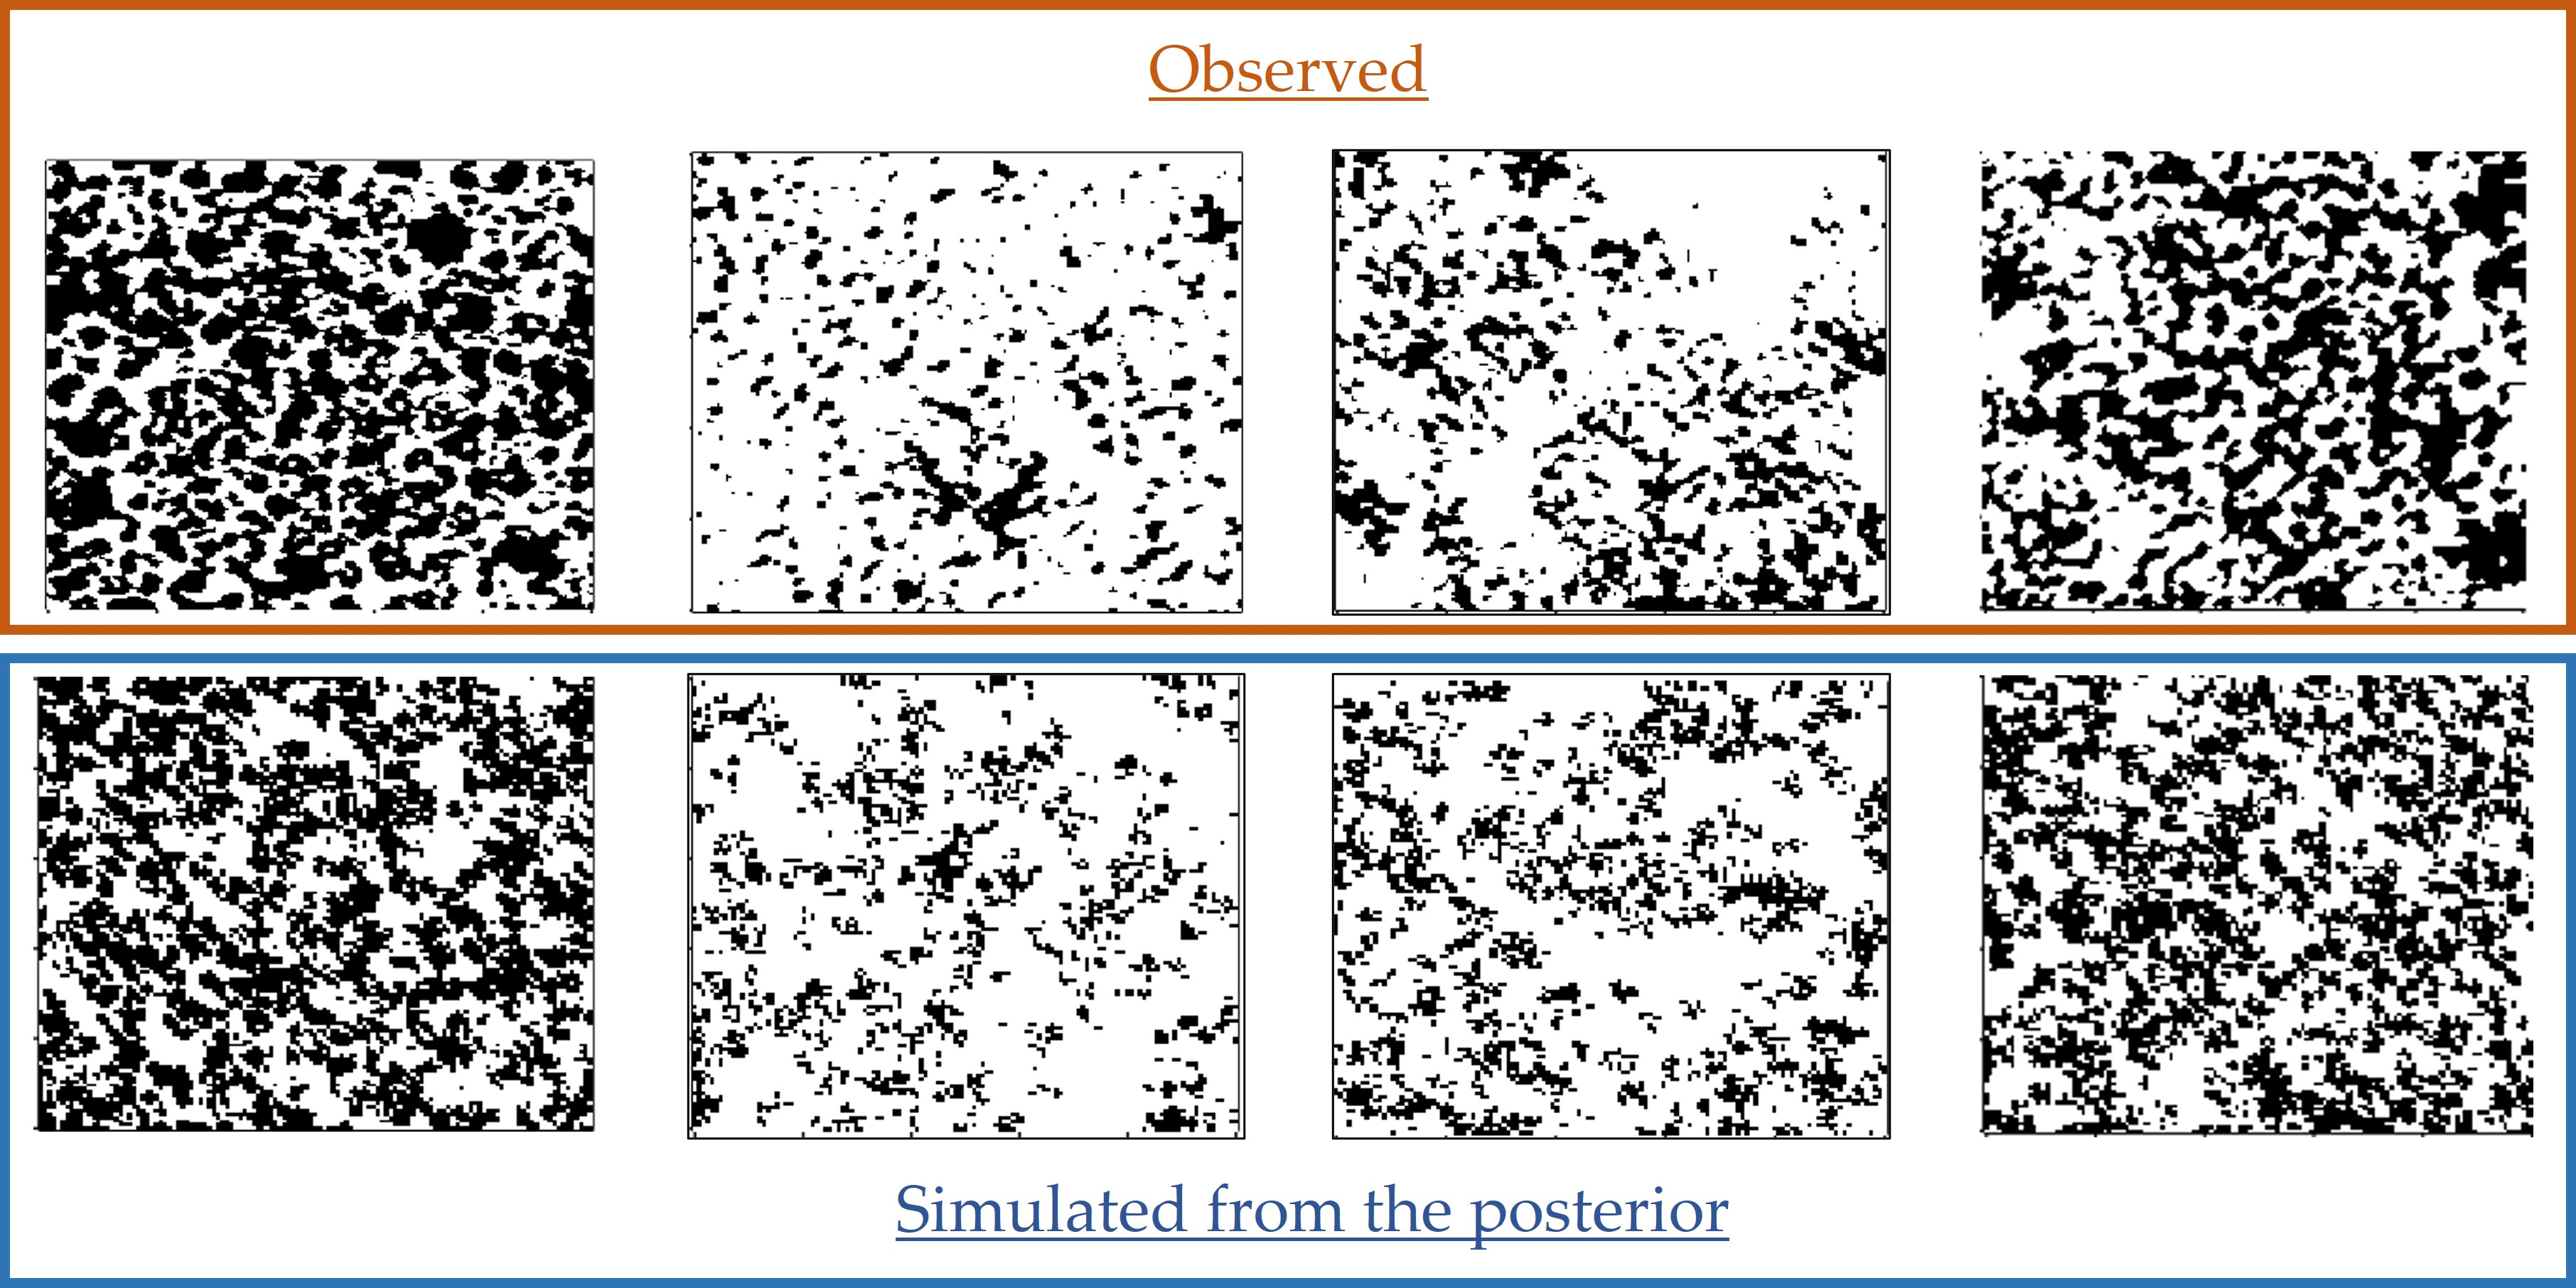
\includegraphics[width=0.8\textwidth]{images/PPC_examples.jpg} 
 
 
 
 
    

}

%====================================================================
\frame{\frametitle{Quand on échoue}
%====================================================================

\centering
    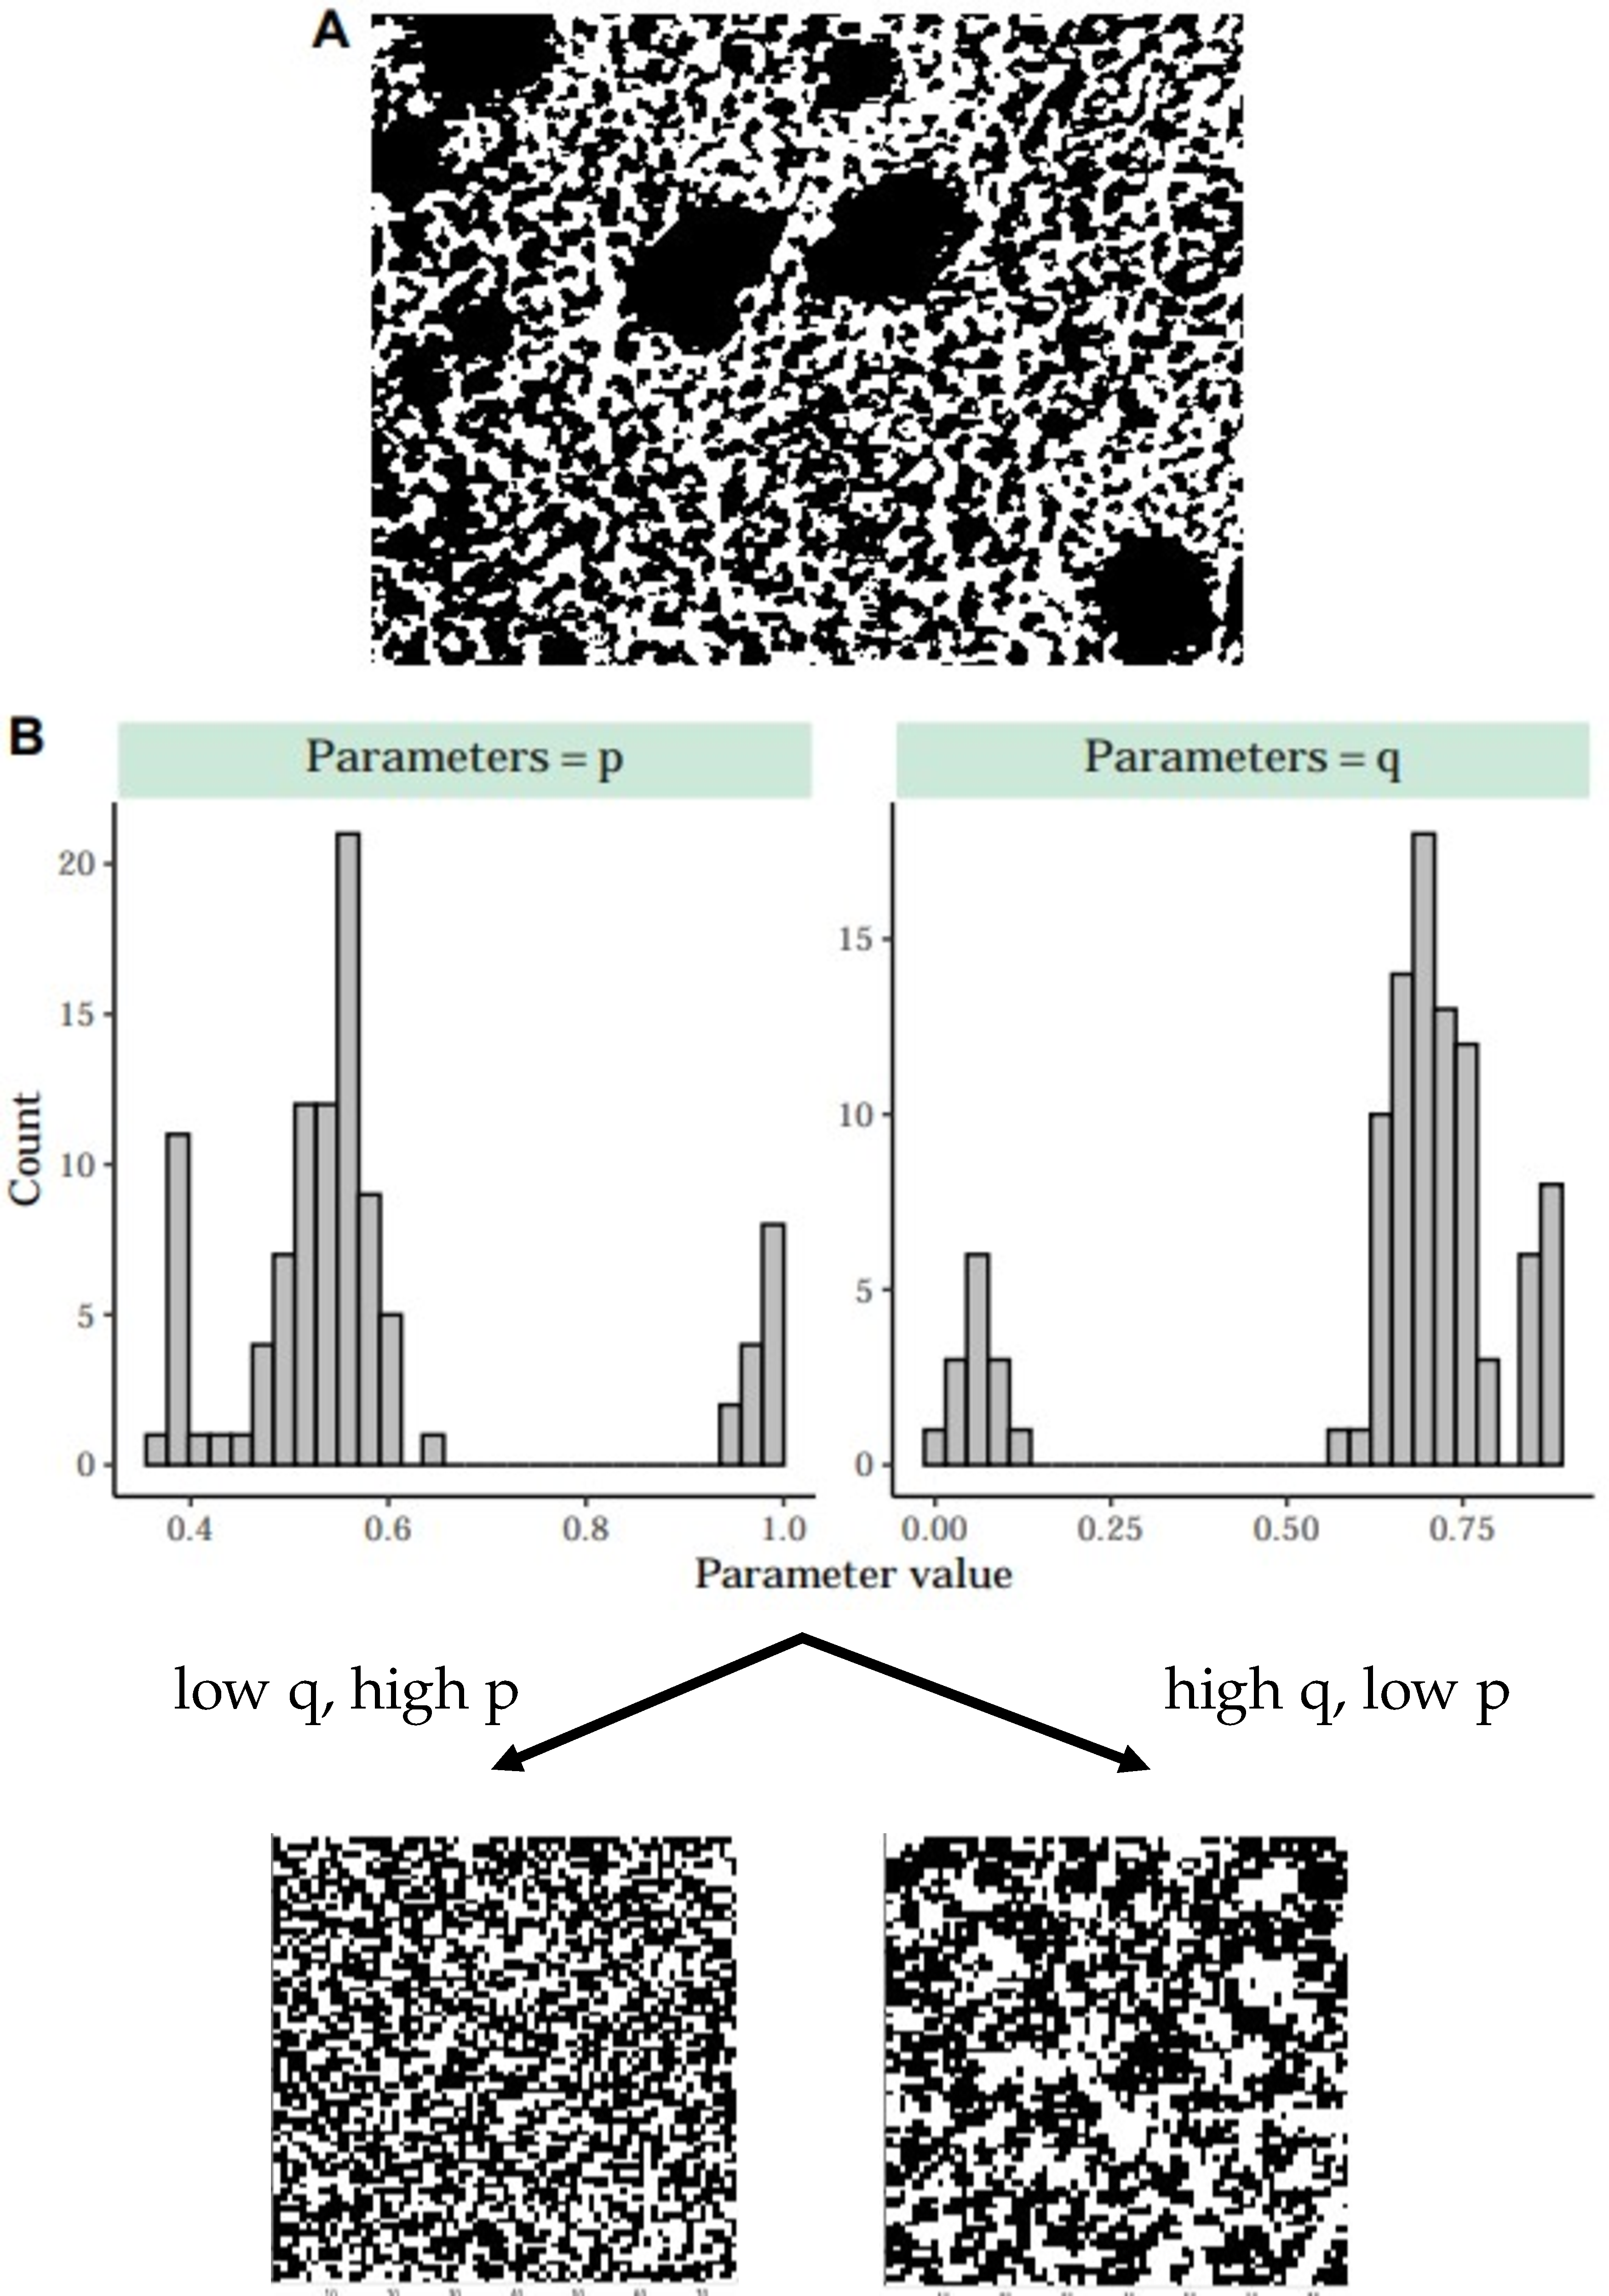
\includegraphics[width=0.5\textwidth]{images/Example_bimodal_distrib} 
 
}

%====================================================================
\frame{\frametitle{Global estimation}
%====================================================================
Considering all the landscapes

\centering
    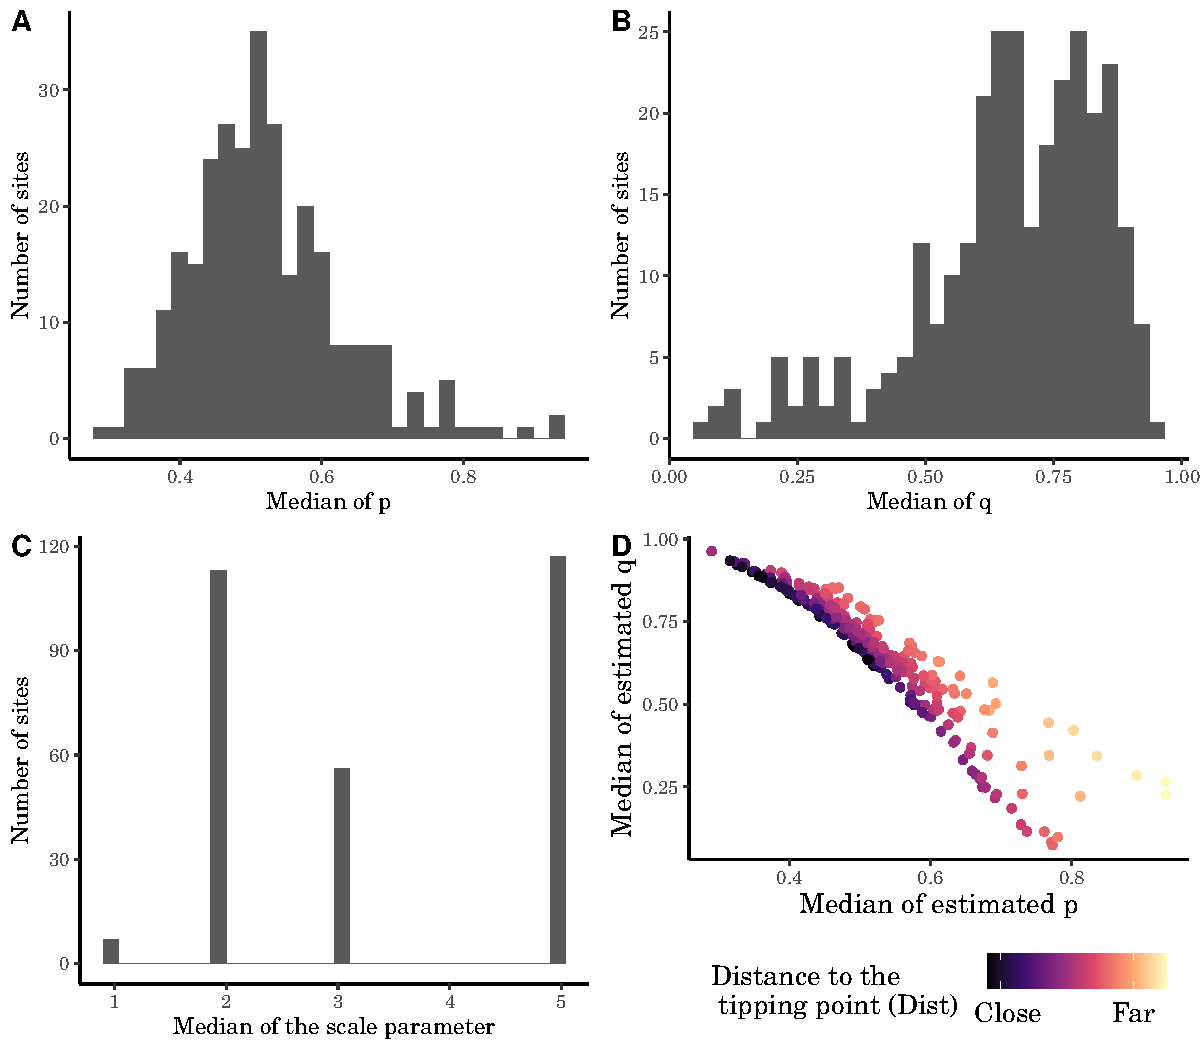
\includegraphics[width=0.8\textwidth]{images/Posterior_median} 
 
}





\section{Prédire le futur de ces écosystèmes}
%====================================================================
\frame{\frametitle{Simuler l'augmentation d'un stress abiotique}
%====================================================================
\begin{itemize}
 \item \textbf{Objectif} : comment les écosystèmes observés évolueront-ils en cas d'augmentation du stress abiotique ? 
 \item \textbf{Scénario} : diminuer le paramètre lié à la reproduction des plantes ($p$).
 \item \textbf{Méthode}
 \begin{itemize}
 \item Pour chaque paysage $\ell$ et échantillon $\theta_{\ell}^{(m)}$ de la distribution postérieure : diminuer $p_{\ell}^{(m)}$ avec des pas fixes ($0.005$) jusqu'à ce que nous ayons atteint une végétation de $0$. 
 \item $p_{\text{crit},\ell}^{(m)}$ : valeur maximale du paramètre $p$ pour laquelle il y a encore de la végétation.  
 \item Distance par rapport au point de désertification
$$
Dist_{\ell}^{(m)} = p_{\ell}^{(m)} - p_{\text{crit},\ell}^{(m)}. 
$$
\end{itemize}

\end{itemize}








}

% %====================================================================
% \frame{\frametitle{Robustness with respect to the model choice}
% %====================================================================
% 
% 
% \centering
%     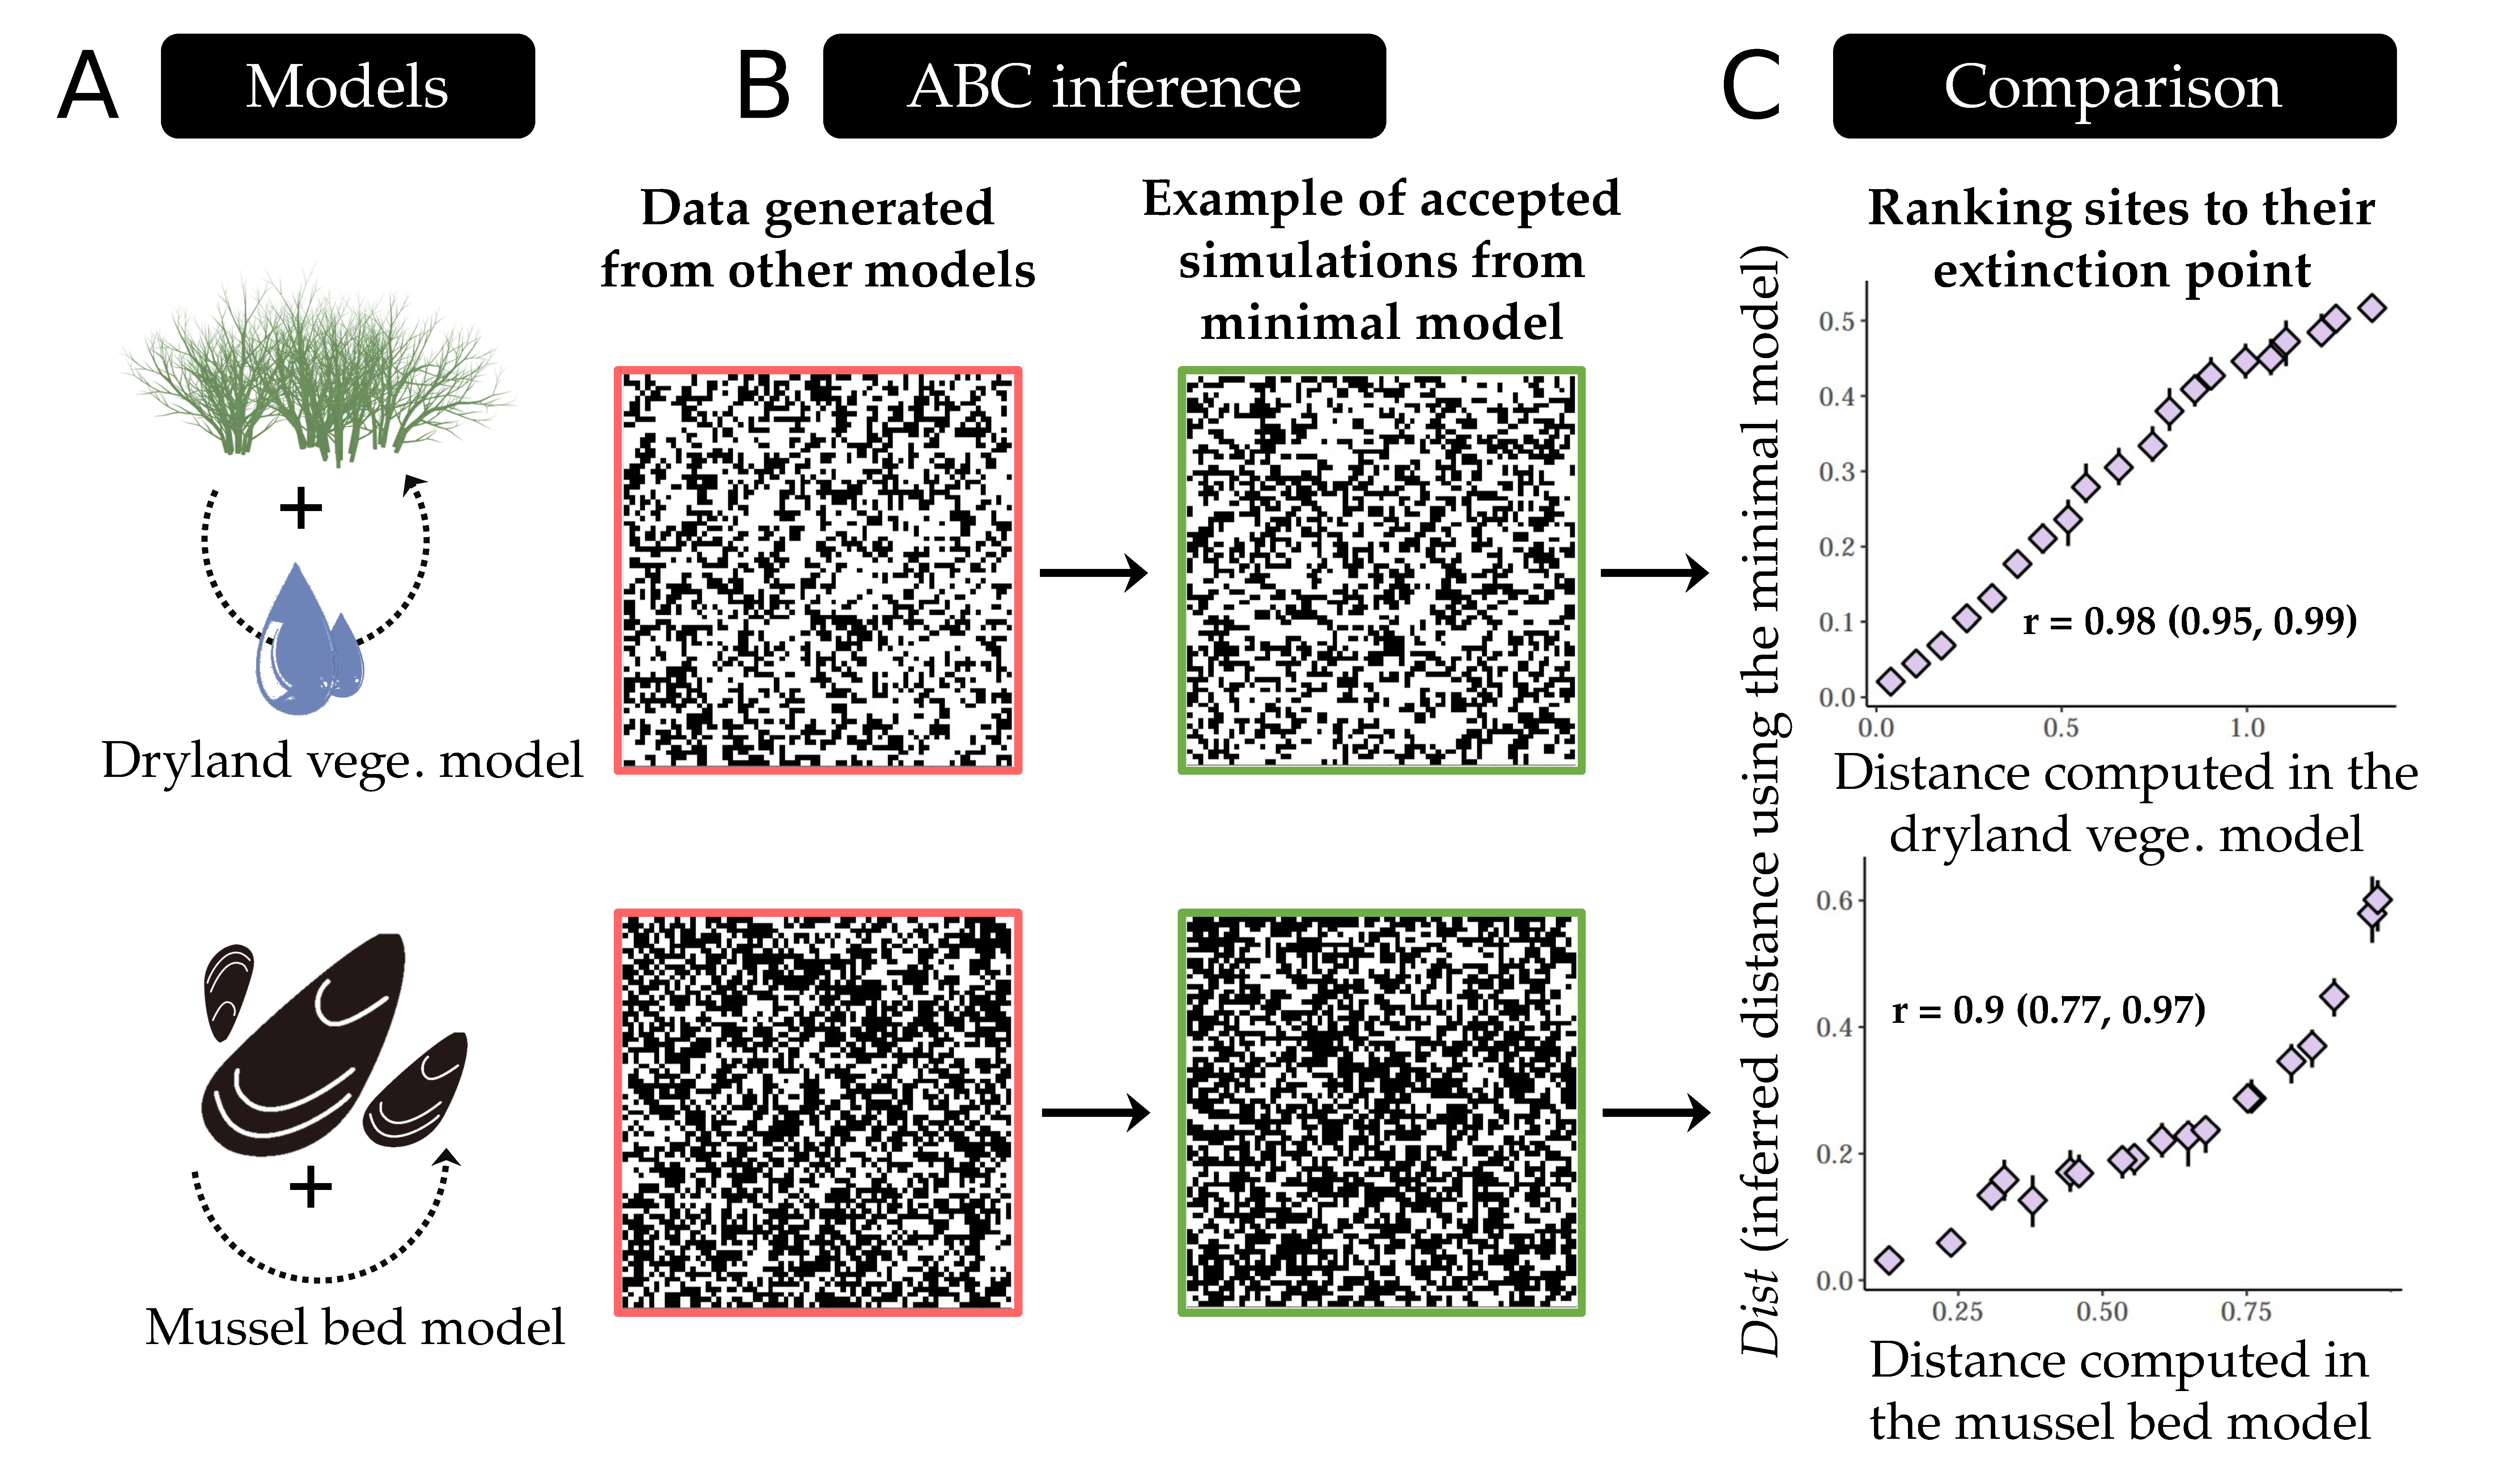
\includegraphics[width=\textwidth]{images/Validation_using_simulations_with_images} 
%  
% 
% 
% 
% }


%====================================================================
\frame{\frametitle{Distance versus projected aridity}
%====================================================================

\centering
    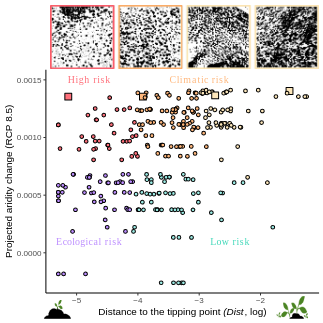
\includegraphics[width=0.7\textwidth]{images/mapping_vulnerability} 

}


%=============================================================
\frame{\frametitle{Conclusion}


\begin{itemize}
 \item Un modèle simple mais identifiable
  \item Première méthode pour comparer la fragilité des écosystèmes
   \item On pourrait vouloir considérer deux tailles de végétation (arbres et herbes)
 \item D'autres pressions telles que le pâturage pourraient être prises en compte ? 
 \end{itemize}
\centering
    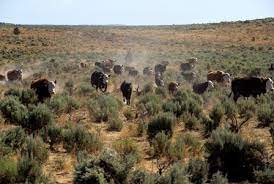
\includegraphics[width=0.5\textwidth]{images/grazing} 

}


%=============================================================
\frame{

\centering


Article soumis : \emph{Estimating distances to tipping points from dryland ecosystem images}, B. Pichon, S. Donnet, I. Gounand, S. Kéfi. \color{blue} \href{https://www.biorxiv.org/content/10.1101/2024.02.20.581244v1}{bioRxiv}

}




\frame[allowframebreaks]{ \frametitle{References}
  {\footnotesize
   %\tiny
   \bibliography{biblio}
   \bibliographystyle{abbrv}
  }
}

%====================================================================
\frame{\frametitle{Prior distribution}
%====================================================================


\centering

$\eta \sim \mathcal{U}_{\{1, \dots,5\}}$ 

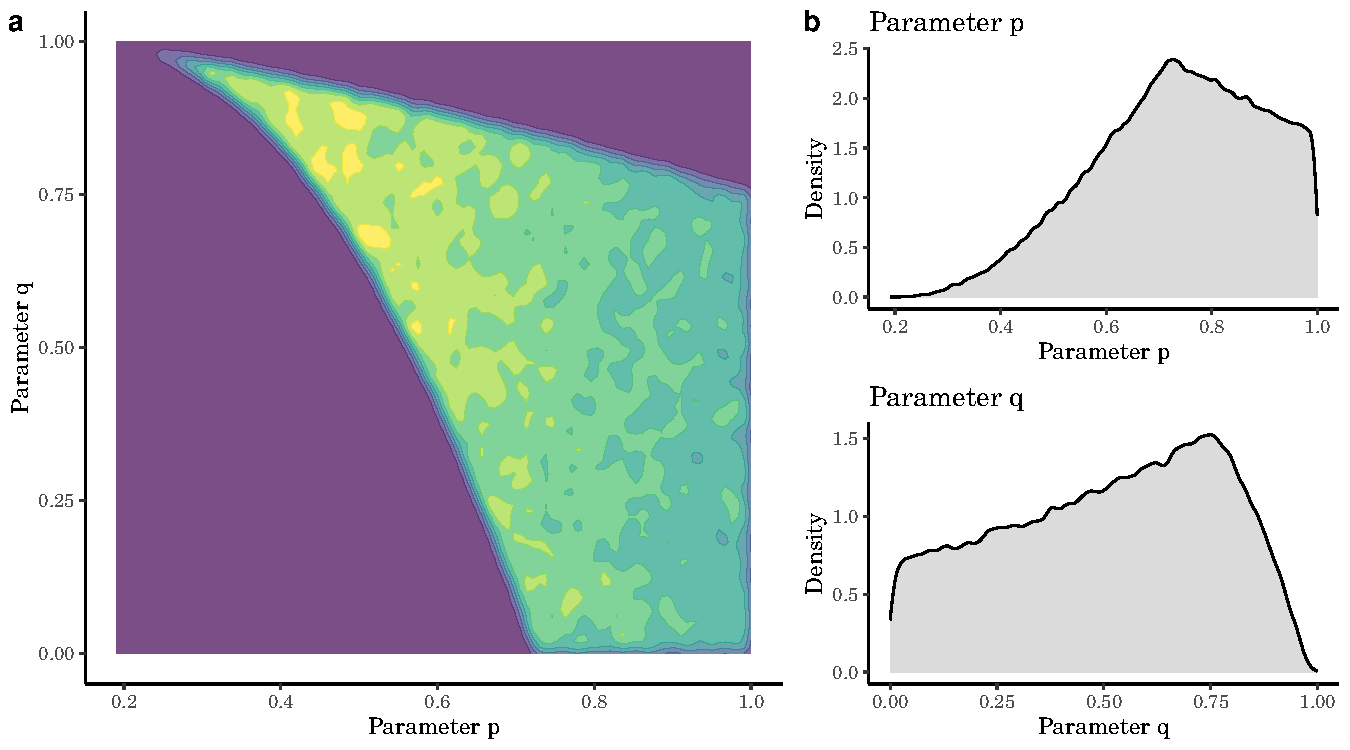
\includegraphics[width = 0.8 \textwidth]{images/Empirical_priors}


Prior ensures that vegetation cover  $\in [0.05,0.9]$


}

\end{document}

  

%====================================================================
%====================================================================


%====================================================================
%====================================================================


